\documentclass[master=mcs]{kulemt}
\setup{
  title={Packed Pre-Constructed Publicly Verifiable Secret Sharing and Applications},
  author={Dheeraj Kumar Suryakari},
  promotor={Prof.\, Nigel P. Smart},
  assessor={Prof.\, Frederik Vercauteren \and Dr.\, Steven Keuchel},
  assistant={Dr.\, Karim Baghery \and Mr.\, Mahdi Rahimi}}
% Remove the "%" on the next line for generating the cover page
%\setup{coverpageonly}
% Remove the "%" before the next "\setup" to generate only the first pages
% (e.g., if you are a Word user).
%\setup{frontpagesonly}

% If you want to include other LaTeX packages, do it here. 
\usepackage{amssymb} % Add this line for \mathbb{}
\usepackage{amsmath} % Add this line for \begin{equation}

\usepackage{amsthm} % Add this line for \begin{theorem}
% \usepackage{amsfonts} % Add this line for \mathbb{}
% \usepackage{graphicx} % Add this line for \includegraphics
\usepackage{caption} % Add this line for \captionof
\usepackage{tcolorbox} % Add this line for \tcolorbox
% \usepackage{graphicx} % Add this line for \includegraphics
% \usepackage{algorithmic}
% \usepackage{algorithmicx}
% \usepackage{algorithm}
\usepackage{float} % Required for [H] specifier
\usepackage{tabularx}
% Finally the hyperref package is used for pdf files.
% This can be commented out for printed versions.
\usepackage[pdfusetitle,colorlinks,plainpages=false]{hyperref}

% \newtheorem{theorem}{Theorem}[section]
\newtheorem{definition}{Definition}[section]
\newtheorem{theorem}{Theorem}[section]
\newtheorem{lemma}{Lemma}[section]
\newtheorem{corollary}{Corollary}[section]
\newtheorem{proposition}{Proposition}[section]
\newtheorem{remark}{Remark}[section]
\newtheorem{example}{Example}[section]

%%%%%%%
% The lipsum package is used to generate random text.
% You never need this in a real master's thesis text!
\IfFileExists{lipsum.sty}%
 {\usepackage{lipsum}\SetLipsumDefault{11-13}}%
 {\newcommand{\lipsum}[1][11-13]{\par And some text: lipsum ##1.\par}}
%%%%%%%

\setcounter{tocdepth}{2} 

%\includeonly{chapter-n}
\begin{document}

\begin{preface}
  I express my gratitude to all those who have supported me throughout my master's thesis 
  journey. I thank my promoter, Prof.\ Nigel P. Smart, for this opportunity and remarks 
  during my mid term presentation. I am grateful to my assessors, Prof.\ Frederik Vercauteren and 
  Dr. Steven Keuchel, for reading and evaluating this thesis report.\par

  Shout out to my daily supervisors, Dr.\ Karim Baghery and Mr.\ Mahdi Rahimi, for their 
  guidance and immense support throughout my thesis work. I had a great time doing the research 
  for my thesis with them, where I learned a lot more about proof systems. I sincerely 
  thank Dr.\ Karim Baghery for explaining some important concepts that were crucial 
  for this thesis and we still have good ideas to explore, hopefully in the future.\par

  Last but not the least, I would like to thank my family and friends for their
  unwavering support and encouragement throughout this journey. I would'nt be here without them.
\end{preface}

\tableofcontents*

\begin{abstract}
  Publicly Verifiable Secret Sharing (PVSS) is one of the popular choices in some applications 
  which require public verifiability when the secret is shared amongst entities. The goal 
  of this thesis is to revisit some applications which can be made more efficient in a 
  secure way using PVSS, for which a new variant of PVSS is proposed in thesis and it is 
  called Packed Pre-Constructed Publicly Verifiable Secret Sharing (PPPVSS or 3PVSS).\par
  
  Firstly, some preliminaries are recalled, followed by a literature review. The 
  sections on preliminaries will give a clear insight into the security properties of 
  the popular Shamir secret sharing which this thesis is based on, and in the section 
  on literature the more recent advancement in PVSS is discussed. Based on 
  the new variant of PVSS proposed in \cite{cryptoeprint:2025/576}, which the authors 
  call it Pre-Constructed Publicly Verifiable Secret Sharing (PPVSS), this thesis 
  proposes 3PVSS which in fact is an extension to PPVSS and gives two practical 
  schemes along with their security proofs.\par

  Approaching to the goal of this thesis, an application is revisited and some changes are proposed 
  using the proposed extension of PPVSS to make it more efficient without 
  compromising much in security.\par
\end{abstract}

% A list of figures and tables is optional
%\listoffigures
%\listoftables
% If you only have a few figures and tables you can use the following instead
\listoffiguresandtables
% The list of symbols is also optional.
% This list must be created manually, e.g., as follows:
\chapter{List of Abbreviations and Symbols}
\section*{Abbreviations}
\begin{flushleft}
  \renewcommand{\arraystretch}{1.1}
  \begin{tabularx}{\textwidth}{@{}p{12mm}X@{}}
    DL & Discrete Logarithm \\
    DLEQ & Discrete Logarithm Equality \\
    PDL & Polynomial Discrete Logarithm \\
    $\mathcal{PPT}$ & Probabilistic Polynomial Time \\
    NIZK   & Non-Interactive Zero Knowledge \\
    PoK   & Proof of Knowledge \\
    AoK  & Argument of Knowledge \\
    PSSS & Packed Shamir Secret Sharing \\
    PVSS & Publicly Verifiable Secret Sharing \\
    PPVSS & Pre-Constructed Publicly Verifiable Secret Sharing \\
    PPPVSS & Packed Pre-Constructed Publicly Verifiable Secret Sharing \\
  \end{tabularx}
\end{flushleft}
\section*{Symbols}
\begin{flushleft}
  \renewcommand{\arraystretch}{1.1}
  \begin{tabularx}{\textwidth}{@{}p{12mm}X@{}}
    $q$ & prime number \\
    $\mathbb{G}$   & Cyclic group of order $q$ \\
    $\mathbb{Z}_q$   & Modular ring with $q$ elements \\
    $\mathbb{Z}_q[X]$  & Univariate polynomial ring in the variable $X$ with coefficients in $\mathbb{Z}_q$ \\
    $\mathbb{Z}_q[X]_t$ & Set of polynomials in $\mathbb{Z}_q[X]$ of degree $t$ \\
    $\mathbb{Z}_q[X]_{\leq t}$ & Set of polynomials in $\mathbb{Z}_q[X]$ of degree at most $t$ \\
    $\lambda$   & Security Parameter \\
    $negl$ & Negligible function \\
    $\mathcal{O}$ & Big-O notation \\
  \end{tabularx}
\end{flushleft}

% Now comes the main text
\mainmatter

\chapter{Introduction}
\label{cha:0}

In this rapidly evolving digital world, cryptography was and is playing a crucial role, which 
allows a user to securely communicate and process sensitive information without any 
fear of eavesdropping or tampering the data. Their whole trust on cryptography boils 
down to their secret keys, which are used to encrypt and/or decrypt their data. In 
reality, however, these secret keys are stored as a whole in their device, making it 
a single point of failure such that an adversary can just steal their secret keys. 
This seriously affects the robustness and availability of the services offered by 
such digital infrastructures. A trivial solution for availability aspect is to make 
multiple copies of the secret keys and store them in multiple devices. However, 
this is not a good idea because now an adversary has multiple points to attack leading 
to decrease in the robustness of the system security. Now one can possibly think to 
divide a given secret key into multiple pieces such that any single piece or up to a 
threshold number of pieces can reveal nothing about the secret key.\par 

In 1979, Shamir introduced a threshold secret sharing scheme called 
Shamir Secret Sharing scheme \cite{10.1145/359168.359176}, which is now a well-known 
and widely used secret sharing scheme to this day because of its numerous applications in
cryptography. Basically, it allows a person to divide their secret into many pieces and distribute 
those pieces amongst other entities, such that a single entity or up to a group of 
entities cannot determine anything about the secret. To reconstruct the secret back, 
one would require more than a threshold number of entity shares. Importantly and interestingly, it is proven to be 
secure against passive adversaries who can see secret shares of some parties and also have 
unlimited computational power.\par 

Shamir secret sharing scheme was first of its kind to have such Information Theoretic (IT) security, 
under certain assumptions, against such passive adversaries. In reality, however, the adversaries 
are usually stronger than just being passive, moreover, they can be active where they 
possess the power to manipulate the share values of the corrupted parties itself. For example, 
an active adversary can manipulate some secret key shares then reconstruction protocol 
for the secret key may yield a wrong secret key, which will badly affect the robustness 
of the system. As Shamir's scheme is not tailored to defend against active adversaries as one cannot 
verify the correctness of the shares, it led to inventing Verifiable 
Secret Sharing (VSS) schemes, which not only does allow the parties to verify the 
correctness of the shares shared by the dealer but also allows the parties to verify 
the correctness of the shares when revealed by the parties during the reconstruction 
phase. This allows VSS schemes to pin point who cheated during the protocol unlike 
in Shamir's scheme which cannot feasibly achieve such functionality. 
Because of the feature of verifiability, VSS schemes found their way into 
many applications which require security against active adversaries.\par

There are many VSS schemes (\cite{d053b0be49644b2f932d703db8c1f8a0}, \cite{DBLP:conf/focs/Feldman87}) 
in the literature which are based on Shamir secret sharing scheme. Throughout the years, many advancements 
have been made in the field of VSS schemes, and as of writing this report the efficient VSS schemes are 
$\Pi_F$, $\Pi_P$ and $\Pi_{LA}$ \cite{cryptoeprint:2023/1669}, each of which have distinct security features. 
In VSS, only shareholders can actually verify the correctness of the shares. Certain applications demand 
to have verifiability feature available to anyone, such is offered by Publicly Verifiable Secret Sharing (PVSS) 
schemes. PVSS is an extension of VSS, where the correctness of the shares can be verified by anyone. Many 
cool applications exist today which use PVSS schemes, such as, e-voting \cite{5581ccd9530540479539d21d1d39ae96}, 
randomness beacons \cite{cryptoeprint:2017/216}, etc. In \cite{cryptoeprint:2025/576}, authors have noticed 
that the Schoenmakers' PVSS scheme used for the e-voting application in \cite{5581ccd9530540479539d21d1d39ae96} 
is actually more than a PVSS scheme, and they coined the term Pre-Constructed Publicly Verifiable Secret Sharing (PPVSS) scheme. 
PPVSS is a special type of PVSS where the dealer additionally publishes a commitment to the secret itself. 
The authors have also shown that any PVSS scheme can be transformed into a PPVSS scheme with minimal 
changes, and constructed a PPVSS $\Lambda_{RO}$ from the PVSS $\Pi_S$ \cite{cryptoeprint:2023/1669} and 
used it to build an efficient e-voting application.\par 

With PPVSS, one can build versatile applications and also can improve the efficiency of existing 
applications. For instance, in ALBATROSS \cite{cryptoeprint:2020/644} authors built a randomness beacon application 
using a PVSS. We have an intuition that an efficient randomness beacon application can be built 
using a scheme based on PPVSS on certain conditions. In this report, we will introduce Packed PPVSS (PPPVSS or 3PVSS), 
an extension of PPVSS where shares representing multiple secrets are secret shared,  
along with its security proofs and give an example based on $\Lambda_{RO}$, which will be used to improve 
ALBATROSS in many cases.\par

The research work presented in this report is based on the following questions:
\begin{itemize}
    \item \textit{What more functionalities can be achieved through PPVSS schemes?}
    \item \textit{How to generalize the PPVSS schemes to the packed version which allows to 
      secret share multiple secrets efficiently?}
    \item \textit{Can we improve the efficiency of some existing applications using PPVSS schemes
      without compromising their security aspects?}
\end{itemize}


\section*{Outline of the thesis}
The next chapter [\ref{chap:preliminaries}] gives the necessary preliminaries required 
to understand the mathematical security guarantees of packed Shamir secret sharing, sigma 
protocols and some examples that were used to build some PVSS and PPVSS schemes. The chapter 
ends with the description of PPVSS scheme and a realtime example of the same. Moving forward, 
chapter \ref{cha:3} introduces packed PPVSS (PPPVSS) scheme and two examples along with 
their security proofs where the proof for latter example is a bit non-trivial. The 
chapter \ref{cha:n} presents a new randomness beacon protocol based on a PPPVSS and 
compares it with the state-of-the-art randomness beacon protocol.
Finally, the chapter \ref{cha:conclusion} concludes the thesis with a summary of the 
results and discusses the possible future work and applications of the PPPVSS scheme.

% In this chapter we sequently recall Packed Shamir secret sharing, 
% Sigma ($\sum$) Protocols and Publicly Verifiable Secret Sharing (PVSS) followed by
% the recent scheme introduced in \cite{cryptoeprint:2025/576}, namely, 
% Pre-Constructed Publicly Verifiable Secret Sharing (PPVSS) which has versatile 
% applications and also improves efficiency in existing applications.
% The agenda of this chapter is to give enough background before describing our Packed PPVSS (PPPVSS) scheme 
% and its corresponding security guarantees in the next chapter.

%%% Local Variables: 
%%% mode: latex
%%% TeX-master: "thesis"
%%% End: 

\chapter{Preliminaries}
\label{chap:preliminaries}

\section{Notation}
Let $(\mathbb{G},\times)$ be a cyclic group of prime order $q$ with hard Discrete Log (DL) and its generator 
being $g$. 
% isomorphic to a subgroup of the multiplicative modular group $\mathbb{Z}_p^*$, where $p$ is prime. 
Also, we write $\mathbb{Z}_{q}[X]_d$ to denote the set of all $d$ degree 
polynomials univariate in $X$ with coefficients in the finite field $\mathbb{Z}_q$. For remainder of the 
chapter we let $n>t$ for some positive integers $n$ and $t$.

\section{Coding Theory}
\label{sec:linear-codes}
This subsection is a brief recall of linear codes and their properties.

\begin{definition}[Codeword]
  A \textbf{codeword} of length $n$ is a vector $c\in \mathbb{Z}_q^n$.
\end{definition}

\begin{definition}[Linear Code]\cite{gallian2024contemporary}
  If $\mathcal{C}$ be a vector subspace of $\mathbb{Z}_q^n$ with dimension $k$, then $\mathcal{C}$ is 
  said to be a \textbf{linear code}(/ linear $q-$ary code) of length $n$ and dimension $k$.
\end{definition}

In the remainder of the subsection, we let $\mathcal{C}$ be a linear $q-$ary code of length $n$ and 
dimension $k$.

\begin{definition}[Hamming distance]
  The hamming distance $d$ of two codewords of equal length is the number of positions at which the 
  codewords differ. Also, the hamming distance of $\mathcal{C}$, $d(\mathcal{C})$ is defined to be the 
  minimum hamming distance of any two codewords in $\mathcal{C}$.
\end{definition}

\begin{definition}[Hamming weight]
  The hamming weight $wt$ of a codeword $c$ is the number of non-zero positions in $c$. Also, the hamming weight of
  $\mathcal{C}$, $wt(\mathcal{C})$ is defined to be the minimum hamming weight of any codeword in $\mathcal{C}$.
\end{definition}

\begin{lemma}\cite{gallian2024contemporary}\label{lem:distance}
  Given a tuple of codewords of equal length $n$, $(u, v, w)$, let $d(u,v)$ and $wt(w)$ denote the hamming 
  distance of $u, v$ and the hamming weight of $w$ respectively. Then $d(u,v) = wt(u-v)$ and 
  $d(u,v)\leq d(u,w)+d(w,v)$.
\end{lemma}

\begin{definition}[error]
  A vector $r$ is said to be an \textbf{error} of a codeword $c\in\mathcal{C}$ if 
  $r=c+e$ for some $e\neq 0$ and $e$ is called error term of $r$.
\end{definition}

It is trivial to observe that the hamming distance of error $r$ of $c\in\mathcal{C}$ is the minimum of the 
hamming distances of $r$ with each codeword in $\mathcal{C}$.

\begin{definition}[Detectable Error]
  An error $r$ of $c\in\mathcal{C}$ is said to be \textbf{detectable} in $\mathcal{C}$ if 
  $r\notin\mathcal{C}$, otherwise it is said to be an \textbf{undetectable}.
\end{definition}

\begin{theorem}\cite{gallian2024contemporary}\label{th:detectable-error}
  An error $r$ of $c\in\mathcal{C}$ is detectable if the hamming distance of $c$ 
  and $r$ is less than the hamming distance of $\mathcal{C}$, more precisely 
  $d(r,c)<d(\mathcal{C})$.
\end{theorem}
\begin{proof}
  Consider the negation of the statement, i.e., the hamming distance of $c$ and $r$ is less than 
  the hamming distance of $\mathcal{C}$ and $r$ is an undetectable error in $\mathcal{C}$, mathematically 
  we have $d(r,c)<d(\mathcal{C})$ and $r\in\mathcal{C}$. The distance of any two codewords in 
  $\mathcal{C}$ should be at least $d(\mathcal{C})$ implying $d(r,c)\geq d(\mathcal{C})$, which is a 
  contradiction to the negation of our statement.
\end{proof}

The theorem \ref{th:detectable-error} says that any error of a codeword in $\mathcal{C}$ is 
detectable as long as their hamming distance is strictly less than the hamming distance of
$\mathcal{C}$ itself.

\begin{definition}[Correctable Error]
  A detectable error $r$ of $c\in\mathcal{C}$ is said to be \textbf{correctable} if one can obtain its 
  error term $e$ such that $c+e=r$.
\end{definition}

\begin{theorem}\cite{gallian2024contemporary}\label{th:correctable-error}
  One can find the error term $e$ of the detectable error $r$ of $c\in\mathcal{C}$ if 
  $wt(e)<\frac{d(\mathcal{C})}{2}$.
\end{theorem}
\begin{proof}
  We have the following triangular inequality from lemma \ref{lem:distance} for any $w\in\mathcal{C}$ with 
  $w\neq c$:
  \begin{align}\label{eq:triangular-inequality}
    d(\mathcal{C})\leq d(w,c)&\leq d(w,r)+d(r,c).
  \end{align}
  From the equation \eqref{eq:triangular-inequality}, we get 
  \begin{align}\label{eq:triangular-inequality-2}
    d(w,r)\geq d(\mathcal{C})-d(r,c).
  \end{align} 
  Since, $w\neq c$ we always will have 
  \begin{align}\label{eq:triangular-inequality-3}
    d(w,r)>d(r,c).
  \end{align}. 
  From the equations \eqref{eq:triangular-inequality-2} and \eqref{eq:triangular-inequality-3}, we have the 
  following result:
  \begin{align*}
    d(\mathcal{C})-d(r,c)>d(r,c) \implies d(\mathcal{C})>2d(r,c) \iff d(\mathcal{C})>2wt(e).
  \end{align*}
\end{proof}

If one wants to correct a detectable error of a codeword in $\mathcal{C}$ then from theorem 
\ref{th:correctable-error}, its hamming distance with the codeword should be strictly less than half 
the hamming distance of $\mathcal{C}$ itself.

\begin{definition}[Dual Code]
  The vector subspace $\mathcal{C}^{\perp}$ is called a Dual (Code) of $\mathcal{C}$ if it is 
  orthogonal to $\mathcal{C}$.
\end{definition}

\begin{definition}[Generating Matrix]
  The $k\times n-$matrix $\mathcal{G}$ is said to be a generating matrix of $\mathcal{C}$ if it 
  generates $\mathcal{C}$, more precisely, the rows of $G$ form a basis for $\mathcal{C}$. Also, $\mathcal{G}$ is said to be in its 
  \textbf{standard form} if it is of the form
  \begin{align*}
    \mathcal{G} = \begin{bmatrix}
      I_k & P
    \end{bmatrix},
  \end{align*}
  where $I_k$ is the $k\times k$ identity matrix and $P$ is some $k\times (n-k)$ matrix.
\end{definition}

\begin{definition}[Parity Check Matrix]
  Consider the linear transformation $\phi$ as follows:
  \begin{align*}
    \phi:& \mathbb{Z}_q^n \rightarrow \mathbb{Z}_q^{n-k},
  \end{align*}
  where kernel of $\phi$ is $\mathcal{C}$. Then the matrix associated to $\phi$, $\mathcal{H}$, 
  is called the \textbf{parity check matrix} of $\mathcal{C}$.
\end{definition}

\begin{lemma}\cite{gallian2024contemporary}
  If $\mathcal{G}$ is a generating matrix of $\mathcal{C}$ in its standard form, i.e., $\mathcal{G} = \begin{bmatrix}
    I_k & P
  \end{bmatrix}$, then $\mathcal{H}$ being a parity check matrix of $\mathcal{C}$ is given by
  \begin{align*}
    \mathcal{H} = \begin{bmatrix}
      -P^T & I_{n-k}
    \end{bmatrix},
  \end{align*}
  where $I_{n-k}$ is the $(n-k)\times (n-k)$ identity matrix where $P^T$ is the transpose of $P$.
\end{lemma}

One can easily check if a codeword is in $\mathcal{C}$ by multiplying it with its corresponding parity 
check matrix $\mathcal{H}$.

\subsection{Reed Solomon Codes}
\label{subsec:reed-solomon}
Consider the set of all univariate polynomials in $X$ of degree at most $t$ over $\mathbb{Z}_q$, denoted by 
$\mathbb{Z}_q[X]_{\leq t}$. It is trivial to observe that $\mathbb{Z}_q[X]_{\leq t}$ is isomorphic to 
the $t+1$ dimensional vector space $\mathbb{Z}_q^{t+1}$, where each vector consists the coefficients of 
a unique polynomial in $\mathbb{Z}_q[X]_{\leq t}$. Now, consider the following set of codewords 
determined by the evaluation of the polynomials in $\mathbb{Z}_q[X]_{\leq t}$ at $n$ \textbf{distinct} 
points $x_1,\dots,x_n\in \mathbb{Z}_q$:

\begin{align}\label{eq:reed-solomon code}
  RS &= \{(f(x_1),\dots,f(x_n)) : f\in \mathbb{Z}_q[X]_{\leq t}, x_i\neq x_j \text{ for }i\neq j\}.
\end{align}  

\begin{lemma}
  Assume $n>t$. The hamming distance of any two codewords in $RS$ is at least $n-t$. Furthermore, $RS$ is 
  a linear code of length $n$ and dimension $t+1$.
\end{lemma}
\begin{proof}
  For $n>t$, saying that the hamming distance of any two codewords is at least $n-t$ is same as saying 
  that the two codewords in $RS$ are equal in at most $t$ positions. Assume by contradiction that 
  there exists two \textbf{distinct} $t$ degree polynomials $f,g$ in $\mathbb{Z}_q[X]$ with corresponding 
  codewords in $RS$ are equal in $t+1$ positions, i.e., their hamming distance is $n-t-1$. As 
  $\mathbb{Z}_q$ is an integral domain, any $t+1$ distinct points in the set 
  $\mathbb{Z}_q\times\mathbb{Z}_q$ will determine a unique $t$ degree polynomial in $\mathbb{Z}_q[X]_t$. 
  As a consequence, we should have $f=g$ in $\mathbb{Z}_q[X]$ which is a contradiction.\par 

  The remainder of the proof is by a consequence of the first part. More precisely, each codeword in 
  $RS$ determined by a polynomial in $\mathbb{Z}_q[X]_{\leq t}$ is actually a unique representation of the 
  polynomial itself as it consists at least $t+1$ distinct evaluations of that polynomial where $n>t$. 
  That is, $RS$ is isomorphic to $\mathbb{Z}_q[X]_{\leq t}$ as a vector space which has dimension $t+1$.
\end{proof}

\begin{definition}[Reed Solomon Code]
  The $q-$ary linear code $RS$ of length $n$ and dimension $t+1$ defined in \eqref{eq:reed-solomon code} 
  with minimum hamming distance $n-t$ is called a \textbf{$[n, t+1, n-t]-$Reed Solomon Code}
  \cite{doi:10.1137/0108018} in $\mathbb{Z}_q$.
\end{definition}

\begin{corollary}\label{cor:detectable-correctable RS}
  All errors in a $[n, t+1, n-t]-$Reed Solomon (RS) code are detectable if their hamming distances with 
  RS are at most $t$ and $2t<n$. Moreover, all errors of hamming distance with RS being at most $t$ can 
  be corrected if $3t<n$.
\end{corollary}
\begin{proof}
  We have that any error of RS has hamming distance at most $t$ with RS. From theorem 
  \ref{th:detectable-error}, any error of a codeword in $RS$ is detectable if its hamming 
  distance is strictly less than the hamming distance of $RS$ itself, i.e., $t<n-t$, which is equivalent 
  to $2t<n$.\par

  To be able to correct the errors of hamming distance at most $t$ with RS, we need $t<\frac{n-t}{2}$ from 
  theorem \ref{th:correctable-error} which is equivalent to $3t<n$.
\end{proof}

In this report, we will use $[n, t+1, n-t]-$Reed Solomon code of the following form:
\begin{align}\label{eq:reed-solomon code-2}
  RS &= \{(f(1),\dots,f(n)) : f\in \mathbb{Z}_q[X]_{\leq t}\}.
\end{align}

\section{Packed Shamir Secret Sharing}
\label{sec:packed-shamir}
$(n,t,\ell)$-Packed Shamir secret sharing (\cite{10.1145/129712.129780},\cite{crypto-1984-905})
 scheme is a threshold secret sharing scheme which is a variant of $(n,t)$-Shamir's 
 secret sharing scheme \cite{10.1145/359168.359176} where $n>2t+\ell-1$. In a nutshell, the $t+\ell-1$ 
 degree secret polynomial with coefficients in $\mathbb{Z}_q$ which evaluates to $\ell$ 
 secrets is secret shared amongst $n$ parties such that any $t+\ell$ parties can 
 reconstruct back the secret polynomial. Recall that Shamir's secret sharing scheme 
 requires at least $t+1$ parties to reconstruct the secret polynomial in contrast to 
 the $t+\ell$ parties in the Packed Shamir secret sharing scheme. The scheme is
 summarized in the Figure \ref{fig:packed-shamir}.
\begin{figure}[ht]
    \centering
    \begin{tcolorbox}[title=\textbf{Packed Shamir Secret Sharing}, width=0.9\textwidth, colframe=blue!75!black, colback=blue!10, sharp corners]
        Given $\ell$ secrets to share amongst $n$ parties, where at most $t$ of them can
        be \textit{(passively)} corrupt, the $(n,t,\ell)$-Packed Shamir secret sharing scheme description is as
        follows:
        
        \vspace{0.5em}
        \textbf{Sharing Algorithm:}
        \begin{itemize}
            \item Dealer constructs the secret polynomial $f\in\mathbb{Z}_q[X]_{t+l-1}$
                  via the lagrange interpolation by choosing $t+\ell$ elements in 
                  $\mathbb{Z}_q$ where $\ell$ of them are secrets, $\{s_i\}_{i=0}^{\ell-1}$, with
                  $f(-i)=s_i$ for all $i$ and remaining $t$ are chosen uniformly 
                  at random in $\mathbb{Z}_q$.
            \item Each party $P_i$ receives their share $f(i)$ from the Dealer
                  for each $i\in\{1,\dots,n\}$
        \end{itemize}
        
        \vspace{0.5em}
        \textbf{Reconstruction Algorithm:}
        \begin{itemize}
            \item Any $\mathcal{Q}$ set containing at least $t+\ell$ parties can use the 
            lagrange interpolation to compute $\{s_i\}_{i=0}^{\ell-1}$ as follows:
            \begin{align*}
                s_m &= \sum_{i\in \mathcal{Q}} f(i) \left[\prod_{j\in \mathcal{Q}, j\neq i}\frac{-m-j}{i-j}\right] &&, m\in\{0,\dots,\ell-1\} \\
            \end{align*}
            \item The secrets $\{s_i\}_{i=0}^{\ell-1}$ are outputted as the result.
        \end{itemize}
    \end{tcolorbox}
    \caption{Packed Shamir Secret Sharing}
    \label{fig:packed-shamir}
\end{figure}

One can observe that all the secret shares of a secret polynomial chosen by the dealer form a codeword in 
$[n,t+\ell,n-t-\ell+1]-$RS code. If the adversary is malicious and can corrupt at most $t$ parties, then from 
corollary \ref{cor:detectable-correctable RS}, the honest shareholders can detect the errors if 
$2t\leq n-\ell$ and moreover all such errors can be corrected if $3t\leq n-\ell$. Also, one can use 
the Berlekamp-Welch algorithm \cite{welch1986error} to correct the errors.\par

But Shamir secret sharing scheme is designed particularly to defend against passive adversaries and not 
against malicious adversaries. A class of threshold secret sharing schemes which are designed to defend 
against malicious adversaries is Verifiable Secret Sharing (VSS). There are many VSS schemes in the literature, 
and as of writing this report the efficient VSS schemes based on Shamir secret sharing are $\Pi_F$, 
$\Pi_P$ and $\Pi_{LA}$ \cite{cryptoeprint:2023/1669} which are alternatives to the original VSS schemes 
from Feldman \cite{DBLP:conf/focs/Feldman87}, Pedersen \cite{crypto-1991-1671} and the more recent 
ABCP \cite{cryptoeprint:2023/992}. VSS schemes based on Shamir secret sharing allow shareholders to 
verify the correctness of the shares obtained during both the sharing and reconstruction phases. This enables 
these VSS schemes to defend against malicious adversaries who can actively corrupt $t$ parties as long as 
$t\leq\frac{n-1}{2}$ (In contrast to $t<\frac{n}{3}$ in Shamir secret sharing). Publicly Verifiable Secret Sharing (PVSS) is an extension of VSS where anyone can 
verify the validity of the secret shares during the sharing phase. More recently, Pre-Constructed Publicly 
Verifiable Secret Sharing (PPVSS)\cite{cryptoeprint:2025/576} was proposed which is an extension of PVSS. 
The main tools used in VSS, PVSS and PPVSS schemes are the \textbf{Zero Knowledge Proofs} which we overview in the 
next section \ref{sec:sigma-protocols}.

\section{Zero Knowledge Proofs}
\label{sec:sigma-protocols}
The agenda of this subsection is to give a brief formal background about some important primitives 
used in the PVSS ,$\Pi_S$ \cite{cryptoeprint:2023/1669}, and the PPVSS ,$\Lambda_{RO}$ \cite{cryptoeprint:2025/576}, schemes. 
A \textit{Zero Knowledge Argument of Knowledge} (ZK AoK)\cite{cryptoeprint:2017/1066} is a protocol between a prover and a verifier
where the prover tries to convince the verifier that a statement is true without revealing any information 
about why it is true. Unlike the Zero Knowledge Proof of Knowledge (ZK PoK) where the prover cannot cheat 
the verifier even with unbounded computational power, a ZK AoK requires the prover to be computationally bounded 
to not be able to cheat any verifier.\par
Let $Y,X$ and $W$ be three sets with $R$ being a ternary relation on $Y\times X\times W$. Consider the 
three PPT interactive algorithms (\textit{Setup}, $P$, $V$), where \textit{Setup} returns a 
common reference string (CRS) $\sigma$ when input $1^{\lambda}$. Given $\sigma$, the following 
is the CRS-dependent language of the relation $R$.
\begin{align*}
  L_{\sigma}=\{x\in X :\exists w\in W, (\sigma, x, w)\in R\},
\end{align*}
where we call $w$ a witness for a statement $x$ if $(\sigma, x, w)\in R$. Also, let $\mathcal{R}$ be 
a PPT algorithm that returns an element in the relation $R$ when input $1^{\lambda}$.\par

Given a relation $R$ and its corresponding language, a \textbf{$\sum$-protocol} 
is a $3$-round \textit{interactive} protocol between two Probabilistic Polynomial Time (PPT) algorithms, 
a prover $P$ 
and a verifier $V$. For some statement in the language of $R$, in the first round $P$ sends a 
commitment $a$ to $V$. To which $V$ sends a challenge $d$ to $P$ in the second round 
and finally $P$ responds back with the response $z$ to $V$ in the third round. 
$V$ outputs \textbf{true} or \textbf{false} upon the proof verification on transcript
$trans := (a, d, z)$. 
Informally, with a $\sum-$protocol a prover $P$ tries to convince
a verifier $V$ that they know a witness $w$ for a given statement $x$ in the language without 
revealing any information about $w$. To state it formally, a $\sum-$protocol is 
supposed to satisfy \textit{completeness}, \textit{Honest Verifier Zero Knowledge} (HVZK)
and \textit{Special Soundness} which are defined as follows.

\begin{definition}[Completeness]
  A $\sum-$protocol is said to be \textbf{complete} for $\mathcal{R}$ if
  the honest verifier $V$ always accepts the honest prover $P$ for any statement in the language 
  defined by $R$.
\end{definition}

\begin{definition}[HVZK]
  A $\sum-$protocol is said to be \textit{Honest Verifier Zero Knowledge}(\textbf{HVZK}) for $\mathcal{R}$ if there exist a PPT algorithm $\mathcal{S}$ 
  that simulates $trans$ of the scheme corresponding to a given statement, $x$, in the 
  language that has witness $w$. 
  That is, given $x$,
  \begin{align*}
    trans(P(x,w)\leftrightarrow V(x)) &\approx trans(\mathcal{S}(x) \leftrightarrow V(x))&& \text{, for any witness $w$ of $x$.}
  \end{align*}
  Where $trans(P(\cdot)\leftrightarrow V(\cdot))$ is the transcript of the $\sum-$protocol amongst 
  $P$ and $V$ and $\approx$ denotes the indistinguishability of the two transcripts.
\end{definition}

\begin{definition}[Special Soundness]
  A $\sum-$protocol is said to satisfy \textbf{Special Soundness} for $\mathcal{R}$, 
  if there exists a PPT extractor $\mathcal{E}$ for any two valid transcripts, $(a,d,z)$ and 
  $(a,d',z')$, corresponding to a given statement $x$ in the language with only a unique 
  witness $w$ and $d\neq d'$ such that $\mathcal{E}(a,d,z,d',z')$ outputs the witness $w$. 
\end{definition}

It is shown that a public-coin, complete, HVZK, special soundness $\sum-$protocol can be made into a
Non Interactive Zero Knowledge (NIZK) Proof of Knowledge (PoK) or Argument of Knowledge (AoK) in the 
Random Oracle ($RO$) model using Fiat-Shamir transform \cite{10.1007/3-540-47721-7_12}. 
In the following subsections, we recall two important NIZK PoK schemes which are used in $\Pi_S$ and 
$\Lambda_{RO}$ schemes. Also, we will introduce a NIZK AoK scheme which will be used in one of 
our new protocols.

\subsection{Chaum-Pedersen Protocol for DL Equality}
\label{subsec:chaum-pedersen}
Recall $\mathbb{G}$ being the cyclic group of prime order $q$ with hard Discrete Logarithm (DL). 
For some $g,h\in \mathbb{G}$ consider the following relation:
\begin{align*}
  R_{DLEQ} &= \{(g,h,a,b),x : a=g^x, b=h^x\}.
\end{align*}
In \cite{10.1007/3-540-48071-4_7}, Chaum and Pedersen proposed a NIZK PoK scheme for the DL Equality 
relation, $R_{DLEQ}$. Informally, a prover $P$ can convince a verifier $V$ that they know $x$ such that
it can be used with both $g$ and $h$ to obtain $a$ and $b$ respectively. This protocol is widely used in
many cryptographic applications like threshold decryption, e-voting and Randomness Beacons. 
We summarize the protocol in Figure \ref{fig:chaum-pedersen}.
\begin{figure}[ht]
    \centering
    \begin{tcolorbox}[title=\textbf{Chaum-Pedersen Protocol for DLEQ}, width=0.9\textwidth, colframe=blue!75!black, colback=blue!10, sharp corners]
        % Let $(g,h,a,b)\in L_{DLEQ}$ be a statement with its corresponding witness being $x$ where $L_{DLEQ}$
        % is the language defined by the relation $R_{DLEQ}$ and 
        Let $g$ be the group generator sampled in the setup phase, $[(g,h,a,b),x]\in R_{DLEQ}$ and 
        $\mathcal{H}$ be a Random Oracle ($RO$).\par
        \vspace{0.5em}
        \textbf{Prover}
        \begin{itemize}
            \item Samples $r\in_{R}\mathbb{Z}_q$ uniformly at random and sets 
                $c_1=g^r$ and $c_2=h^r$.
            \item Sets $d\leftarrow \mathcal{H}(a,b,c_1,c_2)$, where $\mathcal{H}$ is 
                an agreed upon Random Oracle ($RO$).
            \item Sets $z\equiv r+dx \pmod{q}$ and returns the proof(/transcript) $\pi:= (d,z)$.
        \end{itemize}
        
        \vspace{0.5em}
        \textbf{Verifier}
        \begin{itemize}
            \item Checks if $d\leftarrow \mathcal{H}(a,b,\frac{g^z}{a^d},\frac{h^z}{b^d})$ 
                and outputs \textbf{true} or \textbf{false} accordingly.
        \end{itemize}
    \end{tcolorbox}
    \caption{Chaum-Pedersen NIZK PoK for DLEQ}
    \label{fig:chaum-pedersen}
\end{figure}


\subsection{NIZK PoK for Polynomial DL}
\label{subsec:polynomial-dl}
Recall $\mathbb{G}$ being the cyclic group of prime order $q$ with hard Discrete Logarithm (DL) and $g$ 
being its generator. Consider the following relation for some polynomial $f\in\mathbb{Z}_q[X]_t$ with
degree $t<n$:
\begin{align*}
  R_{PDL} &= \{(g,x_1,\dots,x_n,F_1,\dots,F_n),f(X) : (F_i=g^{f(x_i)}, 1\leq i\leq n)\wedge(x_i\neq x_j, i\neq j)\}.
\end{align*}
The $R_{PDL}$ is based on the Polynomial Discrete Logarithm formally introduced in \cite{cryptoeprint:2023/1669}, 
and we recall its definition in the following.

\begin{definition}[Polynomial Discrete Logarithm]
  Let $g$ be a generator for the prime order $q$ cyclic group $\mathbb{G}$. Given $F_1,\dots,F_n$ and distinct elements $x_1,\dots,x_n$ in 
  $\mathbb{Z}_q$, find a polynomial $f\in\mathbb{Z}_q[X]$ with degree at most $t$, where $F_i=g^{f(x_i)}$ 
  for $1\leq i\leq n$ and $t\leq n-1$.\par

  In other words, an algorithm $\mathcal{A}$ is said to have an advantage $\epsilon$ in solving PDL if 
  \begin{align*}
    Pr[\mathcal{A}(x_1,\dots,x_n,g,g^{f(x_1)},\dots,g^{f(x_n)})]\geq\epsilon,
  \end{align*}
  where $f\in\mathbb{Z}_q[X]$ is at most a $t$ degree polynomial with $t\leq n-1$ and the probability is over a 
  chosen random generator $g$ of $\mathbb{G}$ with $q=|\mathbb{G}|$ being prime and distinct $x_1,\dots,x_n$ 
  elements in $\mathbb{Z}_q$.
\end{definition}

\begin{theorem}\cite{cryptoeprint:2023/1669}\label{th:PDL security}
  Let $[(g,x_1,\dots,x_n,F_1,\dots,F_n),f(X)]\in R_{PDL}$ where $f\in\mathbb{Z}_q[X]_{\leq t}$. 
  Assuming PDL is hard, for $0\leq t\leq n-1$, the protocol $\pi_{PDL}$ \ref{fig:polynomial-dl} (described in figure \ref{fig:polynomial-dl}) 
  is a NIZK PoK for $R_{PDL}$ in the $RO$ model.
\end{theorem}

In \cite{cryptoeprint:2023/1669}, Baghery formally introduced a NIZK PoK scheme for the Polynomial DL 
relation, $R_{PDL}$, which is a generalization of Schnorr's ID protocol \cite{crypto-1989-1727}. Informally, 
a prover $P$ can convince a verifier $V$ that they know a $t$ degree polynomial $f$ such that 
it can be used with $g$ to obtain $F_i$ for $1\leq i\leq n$. This protocol is used to construct the PPVSS 
$\Lambda_{RO}$ \cite{cryptoeprint:2025/576}, which was essential in building an efficient e-voting protocol. 
We summarize the protocol in Figure \ref{fig:polynomial-dl}.
\begin{figure}[ht]
    \centering
    \begin{tcolorbox}[title=\textbf{A NIZK PoK for Polynomial DL}, width=0.9\textwidth, colframe=blue!75!black, colback=blue!10, sharp corners]
        Let $(g,x_1,\dots,x_n,F(x_1),F(x_n))\in L_{PDL}$ be a statement with its corresponding witness being $f\in\mathbb{Z}_q[X]_t$ 
        where $L_{PDL}$ is the language defined by the relation $R_{PDL}$.
        
        \vspace{0.5em}
        \textbf{Prover}
        \begin{itemize}
            \item Samples $r\in_{R}\mathbb{Z}_q[X]_t$ uniformly at random and sets 
                $\Gamma_i=g^{r(x_i)}$ for $1\leq i\leq n$.
            \item Sets $d\leftarrow \mathcal{H}(F_1, \dots, F_n, \Gamma_1, \dots, \Gamma_n)$, where $\mathcal{H}$ is 
                an agreed upon Random Oracle (RO).
            \item Sets $z(X)\equiv r(X)+df(X) \pmod{q}$ and returns the proof(/transcript) $\pi:= (d,z(X))$.
        \end{itemize}
        
        \vspace{0.5em}
        \textbf{Verifier}
        \begin{itemize}
            \item First checks if $z$ is a $t$ degree polynomial in $\mathbb{Z}_q[X]_t$. If so, they proceed with the next step.
            \item Checks if $d\leftarrow \mathcal{H}(F_1, \dots, F_n,\frac{g^{z(x_1)}}{F_1^d}, \dots, \frac{g^{z(n)}}{F_n^d})$. 
            \item If first two steps are correct then they output \textbf{true}, otherwise \textbf{false}.
        \end{itemize}
    \end{tcolorbox}
    \caption{A NIZK PoK for Polynomial DL based on Schoenmakers' PVSS}
    \label{fig:polynomial-dl}
\end{figure}


In the next section we will give a brief overview of the Pre-Constructed Publicly Verifiable Secret Sharing 
(PPVSS).

\section{Pre-Constructed Publicly Verifiable Secret Sharing}
\label{sec:ppvss}
Pre-Constructed Publicly Verifiable Secret Sharing (PPVSS) was first introduced in 
\cite{cryptoeprint:2025/576}, which was used as a building block to 
construct an efficient e-voting protocol alternative to Schoenmakers' e-voting protocol. 
Interestingly, the authors in \cite{cryptoeprint:2025/576} observed that the Schoenmakers' e-voting protocol, though 
not efficient in practice, published in 1999 is an unusual application as it is based on a 
PVSS, which led them to discover that the underlying PVSS used is actually a PPVSS. 
What sets PPVSS apart from standard PVSS schemes is that it can be used to build versatile 
applications, such as e-voting, randomness beacons etc., and can 
also improve efficiency of some existing protocols. The subtle difference between PPVSS and 
PVSS is that the secret itself is committed by the prover along with all its corresponding 
secret shares. The relevance of this section is that we will generalize the PPVSS to the case 
where there is more than one secret and use them to revisit a real time application 
to improve its efficiency. Because of its importance in this thesis, we will recall the 
definitions of a PPVSS and an example subsequently.\par

\subsection{Definitions}
\label{sec:ppvss-definitions}

The following definitions are directly taken from \cite{cryptoeprint:2025/576}.

\begin{definition}[PPVSS]
    A PPVSS scheme should have four algorithms, namely, Initial, Share, Verify and Reconstruction whose 
    descriptions are as follows:
    \begin{itemize}
        \item \textbf{Initial} $(1^\lambda)\rightarrow(\{PK_i,SK_i\}_{i=1}^n\sqcup\{h_0\text{ or }(PK_0,SK_0)\})$: 
          When given $1^\lambda$, each party $P_i$ for $1\leq i\leq n$ registers their public key $PK_i$ in a 
          public ledger and withholds the corresponding secret key $SK_i$. Also, all parties and the dealer $D$ 
          agree on a commitment key or public key whose secret key is known to a target person. 
          Note that the message space of the public-key scheme is a subgroup of $(\mathbb{G},\times)$.
        \item \textbf{Share} $(n,t,f_0,\{PK_i\}_{i=1}^n\bigsqcup\{h_0\text{ or }PK_0\})$\par
          $\rightarrow(\{y_i\}_{i=0}^n,\pi_{PPVSS})$:\par 
          It secret shares $f_0$ to obtain the shares $\{f_i\}_{i=1}^n$. For $1\leq i\leq n$, uses 
          the public key $PK_i$ to encrypt $f_i$ and obtain the encrypted share $y_i$. Now, it uses the commitment 
          key $h_0$ ( or public key $PK_0$) to commit(/encrypt) $f_0$ to obtain $y_0$. 
          In the next step, it uses a NIZK proof $\pi_{PPVSS}$ protocol to prove that $y_0$ is a valid 
          commitment(/encryption) of the secret and $\{y_i\}_{i=1}^n$ has valid encryptions of the corresponding shares. Finally, it returns $(\{y_i\}_{i=0}^n,\pi_{PPVSS})$.\par
        \item \textbf{Verify} $(n,t,\{y_i\}_{i=0}^n,\pi_{PPVSS})\rightarrow$ \textbf{true/false}: 
          This algorithm(which can be performed by anyone) checks if the NIZK proof $\pi_{PPVSS}$ is valid for 
          $\{y_0,\dots,y_n\}$ and then returns true, otherwise false.\par
        \item \textbf{Reconstruct}: There are two approaches based on cooperation of the dealer $D$ and are as follows:
          \begin{itemize}
            \item \textbf{(Optimistic)} $Reconstruction^{opt}[\{h_0,f_0,r_0,y_0\}\text{ or }\{PK_0,SK_0,y_0\}]$\par$\rightarrow(f_0\text{ or }false)$:
              
              Given the input a verifier checks if $y_0$ is a valid commitment(/encryption) of the secret. 
                 If so, it returns $f_0$; otherwise it returns $false$.
            \item \textbf{(Pessimistic)} $Reconstruction^{pes}[\{y_i,SK_i\}_{i\in\mathcal{Q},|\mathcal{Q}|=t+1}]\rightarrow(f_0\text{ or }false)$: 
              Given any $t+1$ encrypted shares along with corresponding secret keys, it outputs the secret 
              $f_0$ or $false$. This can be done in two phases as follows: 
                \begin{itemize}
                  \item \textbf{Decryption of the shares}, each party $P_i\in\mathcal{Q}$ decrypts $y_i$ to obtain 
                    $f_i$ using its secret key $SK_i$. Then it generates a NIZK proof $\pi_i^{Dec}$ which proves that 
                    $f_i$ is the correct decryption of $y_i$. Now, $P_i$ publishes $(f_i,\pi_i^{Dec})$.
                  \item \textbf{Share pooling}, a verifier $V$ (not necessarily from the shareholders) checks if proof 
                   $\pi_i^{Dec}$ is correct for each $P_i\in\mathcal{Q}$. If any check fails, then $V$ returns $false$; 
                   otherwise $V$ applies a reconstruction procedure to the set of valid shares, $\{f_i\}_{i\in\mathcal{Q},|\mathcal{Q}|=t+1}$, 
                   and returns $f_0$.
                \end{itemize}
          \end{itemize}
    \end{itemize}
\end{definition}

A PPVSS is said to be secure:

\begin{itemize}
  \item \textbf{Correctness}: If the dealer and parties follow the protocol, then the \textit{\textbf{Verify}} 
    algorithm returns \textit{\textbf{true}} and the \textit{\textbf{Reconstruct}} algorithm returns $f_0$ 
    irrespective of which approach. For any integer $n\geq t+1$ with $t\geq0$, a PPVSS is said 
    to be correct for
    $\left(\{PK_i,SK_i\}_{i=1}^n\sqcup\{h_0\text{ or }(PK_0,SK_0)\}\right)\leftarrow$\textbf{Initial} $(1^\lambda)$ when 
    it satisfies the following based on the output of the \textit{Share} algorithm.\par
   When \textit{Share} algorithm outputs a commitment(/encryption) of the secret, then
        \begin{align*}
          Pr\begin{bmatrix}
            (\{y_i\}_{i=0}^n,\pi_{PPVSS})&\leftarrow \textit{\textbf{Share}} \big(n,t,f_0,\{PK_i\}_{i=1}^n\bigsqcup\\
            &\{h_0\text{ or }PK_0\}:\\
            \textit{\textbf{true}}&\leftarrow \textit{\textbf{Verify}} (n,t,\{y_i\}_{i=0}^n,\pi_{PPVSS})
          \end{bmatrix} = 1,
        \end{align*}
    
        \begin{align*}
          Pr\begin{bmatrix}
            (\{y_i\}_{i=0}^n,\pi_{PPVSS})&\leftarrow \textit{\textbf{Share}} \big(n,t,f_0,\{PK_i\}_{i=1}^n\bigsqcup\\
            &\{h_0\text{ or }PK_0\}),\\
            f_0^{'}&\leftarrow Reconstruction^{opt}[\{h_0,f_0,r_0,y_0\}\\
            &\textit{ or }\{PK_0,SK_0,y_0\}\bigvee\\
            f_0^{'}&\leftarrow Reconstruction^{pes}[\{y_i,SK_i\}_{i\in\mathcal{Q},|\mathcal{Q}|=t+1}]:\\
            &f_0^{'}=f_0
          \end{bmatrix} = 1.
        \end{align*}
  \item \textbf{Verifiability}: If \textit{\textbf{Verify}} returns \textit{\textbf{true}}, then 
    \textit{\textbf{(Optimistic)}} $Reconstruct^{opt}$ and/or \textit{\textbf{(Pessimistic)}} $Reconstruct^{pes}$ 
    output being $f_0$ is the actual secret of whom the shares are encrypted. Moreover, 
    $\{y_i\}_{i=1}^n$ are valid encryptions of the shares of same secret with 
    high probability if the following statement is true.\par
    $y_0$ is a valid commitment(/encryption) of the secret with high 
        probability. More formally, given $\lambda$, for any integers 
        $n\geq 2t+1$ and $t\geq0$, a PPVSS is said to be verifiable if for any 
        $\mathcal{PPT}$ adversary $\mathcal{A}$, we have:
        \begin{align*}
          Pr\begin{bmatrix}
            \big(\{PK_i,SK_i\}_{i=1}^n\sqcup&\{h_0\text{ or }(PK_0,SK_0)\}\big)\leftarrow\textbf{ Initial } (1^\lambda),\\
            (\{y_i\}_{i=0}^n,\pi_{PPVSS})&\leftarrow \mathcal{A} \big(n,t,f_0,\{PK_i\}_{i=1}^n\bigsqcup\\
            &\{h_0\text{ or }PK_0\}\big),\\
            f_0^{'}&\leftarrow Reconstruction^{opt}[\{h_0,f_0,r_0,y_0\}\\
            &\textit{ or }\{PK_0,SK_0,y_0\}]\bigvee\\
            f_0^{'}&\leftarrow Reconstruction^{pes}[\{y_i,SK_i\}_{i\in\mathcal{Q},|\mathcal{Q}|=t+1}]:\\
            \textit{\textbf{true}}&\leftarrow \textit{\textbf{Verify}} (n,t,\{y_i\}_{i=0}^n,\pi_{PPVSS})
            \bigwedge f_0^{'}\neq f_0
          \end{bmatrix} \leq negl(\lambda),
        \end{align*}
        where $\mathcal{Q}$ is the set of honest parties.
  \item \textbf{IND1-Secrecy (Indistinguishability of Secrets)}: Before reconstruction phase, any amount of public 
    information along with secret keys of at most $t$ parties excluding $SK_0$ will give 
    absolutely no information about the secret $f_0$. More formally, for integers $n>1$ and 
    $t+1\leq n$, the PPVSS is said to satisfy \textit{IND1-Secrecy} if for any $\mathcal{PPT}$ adversary $\mathcal{A}$ 
    corrupting at most $t$ parties, excluding the owners of $SK_0$, has negligible 
    advantage in the following game played against a challenger.
    \begin{itemize}
      \item The challenger runs \textit{\textbf{Initial}} $(1^\lambda)$ of PPVSS to obtain 
        $\{PK_i,SK_i\}_{i=1}^n\sqcup\{h_0\text{ or }(PK_0,SK_0)\}$ and sends all public 
        information along with secret information of all corrupted parties to $\mathcal{A}$.
      \item The challenger chooses two secrets, $s_0=f_0$ and 
        $s_1=f_0^{'}$ at random in the space of secrets. Furthermore, it chooses $b\in\{0,1\}$ 
        uniformly at random and runs 
        \textit{\textbf{Share}} $(n,t,s_0,\{PK_i\}_{i=1}^n\bigsqcup\{h_0\text{ or }PK_0\})$ 
        algorithm of the PPVSS scheme and obtains $(\{y_i\}_{i=0}^n,\pi_{PPVSS})$. Finally, it 
        sends all public information generated in \textit{Share} phase together with $s_b$.
      \item $\mathcal{A}$ guesses a bit $b'\in\{0,1\}$.
    \end{itemize}
    The advantage of $\mathcal{A}$ is defined to be $|Pr[b'=b]-\frac{1}{2}|$.
\end{itemize}

We now will recall 
$\Lambda_{RO}$, the PPVSS scheme introduced in \cite{cryptoeprint:2025/576} which is actually based on 
$\Pi_S$ \cite{cryptoeprint:2023/1669} in figure \ref{fig:ppvss}.\par 
\begin{figure}[ht]
    \centering
    \resizebox{\textwidth}{!}{ % Further reduced the scaling factor to fit the content
    \begin{tcolorbox}[title=\textbf{$\Lambda_{RO}$ \cite{cryptoeprint:2025/576}}, width=1.2\textwidth, colframe=blue!75!black, colback=blue!10, sharp corners]
        
        \textbf{Initialization:}
            All parties $\{P_i\}_{i=1}^n$ and dealer $D$ agree on the prime field $\mathbb{Z}_q$, a group $(\mathbb{G},\times)$ of 
            order $q$ with a generator $g$, random oracle $\mathcal{H}$. Also, each party 
            $P_i$ registers their public key $PK_i$ in the public ledger and all agree on a commitment 
            key or a public key, $PK_0\neq g$, whose secret key is known to a target person.

        \vspace{0.5em}
        \textbf{Share:}
        \begin{itemize}
            \item Dealer $D$ samples a $t$-degree polynomial $f\in\mathbb{Z}_q[X]$ uniformly at random and 
              sets $g^{f_0}$ as the secret to be shared, where $f_0=f(0)$.
            \item For each $1\leq i\leq n$, $D$ computes $f(i)=f_i$ and uses $PK_i$ to encrypt the secret share  
               to obtain $PK_i^{f_i}=y_i$. $D$ also encrypts(/commits) to the secret $g^{f_0}$ using the encryption(/commitment) 
              key $PK_0$ to obtain $y_0=PK_0^{f_0}$. 
            \item $D$ uses the PDL proof scheme \ref{subsec:polynomial-dl} to generate $\pi_{PDL}$ as follows:
                 \begin{itemize}
                    \item Samples a $t-$degree polynomial $r\in\mathbb{Z}_q[X]$ uniformly at random and 
                    computes $c_i=PK_i^{r_i}$ where $r_i=r(i)$ for $0\leq i\leq n$.
                    \item Using $\mathcal{H}$, $d=\mathcal{H}(y_0,\dots,y_n,c_0,\dots,c_n)$ is computed.
                    \item Sets $z(X)=r(X)+df(X)$, hence $\pi_{PDL}=(d,z(X))$ is obtained. 
                 \end{itemize}
            \item $D$ broadcasts the encryptions of the shares along with the encryption(/commitment) of the secret 
              with $\pi_{PDL}$ which proves the validity of the encrypted shares and encrypted(/committed) 
              secret, i.e., broadcasts $\{y_i\}_{i=0}^n$ and $(d,z(X))$.
        \end{itemize}
        
        \vspace{0.5em}
        \textbf{Verification:}
            Given public keys $\{PK_i\}_{i=1}^n$ and public(commitment) key $PK_0$, any entity can check 
            $\pi_{PDL}$ to verify the correctness of the encrypted shares $\{y_i\}_{i=1}^n$ and $y_0$ being the encryption(/commitment) of the secret. 
            They will output \textbf{true} or \textbf{false} based on the verification of the proof. The 
            procedure is outlined as follows:
        \begin{itemize}
            \item The entity checks if $z(X)$ is a $t-$degree polynomial or not.
            \item Checks if $d=\mathcal{H}(y_0,y_1,\dots,y_n,\frac{PK_0^{z(0)}}{y_0^d},\frac{PK_1^{z(1)}}{y_1^d},\dots,\frac{PK_n^{z(n)}}{y_n^d})$.
            \item Outputs \textbf{true} if both of the above checks are satisfied, otherwise \textbf{false}.
        \end{itemize}

        \vspace{0.5em}
        \textbf{Reconstruction:}
            There are two approaches to reconstruct the secret $g^{f_0}$ based on the 
            cooperation of the dealer $D$ which are as follows:
            \begin{itemize}
                \item \textbf{Optimistic Reconstruction:} $D$ publishes $f_0$, then any verifier (not necessarily shareholders) 
                when given $g,PK_0,y_0$ can check if $y_0=PK_0^{f_0}$ and returns $g^{f_0}$ 
                if the check passes, if not they return \textbf{false}.
                \item \textbf{Pessimistic Reconstruction:} If $D$ refuses to reveal $f_0$, then any set 
                $\mathcal{Q}$ consisting at least $t+1$ shareholders will do the following (which 
                is same as the reconstruction step in the PVSS $\Pi_S$ protocol):
                \begin{itemize}
                    \item Each party $P_i\in\mathcal{Q}$ decrypts their share $y_i$ using their private key $SK_i$ 
                      corresponding to $PK_i$ to obtain $g^{f_i}$. Then they publish $g^{f_i}$ 
                      along with a DLEQ proof \ref{subsec:chaum-pedersen}, $\pi_{DLEQ}$ which proves that the 
                       $g^{f_i}$ is the correct decryption of $y_i$.
                    \item If $\mathcal{Q}$ consists at least $t+1$ honest parties, they can use the 
                    lagrange interpolation to compute the secret $g^{f_0}$ as follows:
                    \begin{align*}
                        g^{f_0} &= \prod_{i=1}^{t+1} g^{f_i^{\lambda_i}} = g^{\sum_{i=1}^{t+1}f_i\cdot\lambda_i},\\
                    \end{align*}
                    where $\lambda_i=\prod_{j\neq i}\frac{j}{j-i}$ are lagrange coefficients.
                \end{itemize}
            \end{itemize}
    \end{tcolorbox}
    }
    \caption[PPVSS Scheme]{a Pre-Constructed Publicly Verifiable Secret Sharing (PPVSS) scheme}
    \label{fig:ppvss}
\end{figure}
The security guarantees of $\Lambda_{RO}$ are explained in \cite{cryptoeprint:2025/576} which follows from 
the security guarantees of $\Pi_S$, also the authors used $\Lambda_{RO}$ to build a new e-voting 
protocol alternative to the replaced Schoenmakers' e-voting protocol \cite{5581ccd9530540479539d21d1d39ae96} 
and showed that they achieved improvement in the verification phase 
(7 to 30 times faster in implementation for some parameters). 

\section{Conclusion}
In summary, we recalled some basic concepts of linear codes and Reed Solomon codes as an example. We then 
recalled the Packed Shamir secret sharing scheme which is a generalization of the Shamir Secret Sharing scheme \cite{10.1145/359168.359176} 
that was originally designed to defend against passive adversaries and showed its correspondence with 
Reed Solomon codes. As one of the goals of this thesis is to explore threshold secret sharing schemes that commits to 
secret and also 
can defend against malicious adversaries, we briefly recalled PPVSS \cite{cryptoeprint:2025/576}. 
Moving forward, in the next chapter we will introduce 
Packed Pre-Constructed Publicly Verifiable Secret Sharing (PPPVSS) which is a generalization of 
PPVSS and give two examples whose inspiration is drawn from $\Lambda_{RO}$.

%%% Local Variables: 
%%% mode: latex
%%% TeX-master: "thesis"
%%% End: 

%\chapter{More efficient PVSS and PPVSS}
\label{cha:2}
This chapter introduces a new PVSS scheme that is more efficient in terms of verification time 
than the state-of-the-art PVSS $\Pi_{S}$ \cite{cryptoeprint:2023/1669}. We noticed that the 
PVSS version where the secret is $g^{f_0}$ can never be secure against a malicious dealer who 
has access to unbounded computational power. This is because a computationally unbounded 
dealer can always cheat shareholders by giving them a fake proof of knowledge about the 
public-key encryptions of the secret.\par 

Due to this reason, we can use ZK AoK proof systems to improve the overall efficiency of 
PVSS schemes. In the remainder of this chapter, we will introduce a new NIZK AoK proof system 
and use it to construct a new PVSS scheme which is based on $\Pi_S$. As a consequence, 
we will also give a new PPVSS scheme.

\section{NIZK AoK for Polynomial DL}
\label{sec:AoK_R_pdl}
Consider the set $\{g_i\}_{i=1}^n$ containing $n$ distinct generators (obtained as CRS) of 
the prime order $q$ cyclic group $\mathcal{G}$ different from $g$, where $n<\varphi(q)$ and $\varphi(q)$ is 
the total number of distinct generators of the cyclic group $\mathbb{G}$. Consider the following relation for 
some polynomial $f\in\mathbb{Z}_q[X]_{t}$ with $0\leq t< n$:
\begin{align}\label{eq:relation_mod_PDL_ultimate}
  R_{PDL}^{mod} = \{(g_1,\dots,g_n,g,x_1,\dots,x_n,F_0,&\dots,F_n),f(X) : F_0=\prod_{i=1}^{n}g_i^{f(x_i)},\\\nonumber &F_i=g^{f(x_i)}, 1\leq i\leq n\},
\end{align}
where all $x_i$'s are distinct in $\mathbb{Z}_q$. The $R_{PDL}^{mod}$ is inspired from $R_{PDL}$ 
\cite{cryptoeprint:2023/1669} recalled in subsection \ref{subsec:polynomial-dl}. As a consequence, 
it is based on the following \textit{modified} PDL problem.

\begin{definition}[modified PDL problem]
  Let $g,g_1,\dots,g_n$ be distinct group generators of $\mathbb{G}$ of order $q$. 
  Given $\mathbb{F}\in\mathbb{G}$ and distinct elements $x_1,\dots,x_n$ in $\mathbb{Z}_q$, find 
  a polynomial $f(X)\in\mathbb{Z}_q[X]_t$ of at most degree $t$ such that 
  $F_0=\prod_{i=1}^{n}g_i^{f(x_i)}$ and $F_i=g^{f(x_i)}$ for $1\leq i\leq n$ where $0\leq t<n$.\par

  In other words, an algorithm $\mathcal{A}$ has advantage $\epsilon$ in solving the modified PDL problem in 
  $\mathbb{G}$ if:
  \begin{align*}
    \Pr[\mathcal{A}(x_1,\dots,x_n,g,g_1,\dots,g_n,\prod_{i=1}^{n}g_i^{f(x_i)},g^{f(x_1)},\dots,g^{f(x_n)})=f(X)]\geq \epsilon,
  \end{align*}
  where $f$ is at most a $t$ degree polynomial in $\mathbb{Z}_q[X]$ with $0\leq t<n$. The 
  probability is taken over distinct $x_i$'s in $\mathbb{Z}_q$, and the random with distinct 
  generators $g,g_1,\dots,g_n$ of $\mathbb{G}$.
\end{definition}

Consider the CRS dependent language of $R_{PDL}^{mod}$ as follows:
\begin{align*}
  L_{g_1,\dots,g_n}^{mod-PDL} = \{(g,x_1,\dots,x_n,&F_0,\dots,F_n) :\\ &\exists f\in\mathbb{Z}_q[X]_t, [(g_1,\dots,g_n,g,x_1,\dots,x_n,F_0,\dots,F_n),f(X)]\in R_{PDL}^{mod}\}
\end{align*}
We now present our NIZK AoK proof system $\pi_{PDL}^{mod}$ for the relation $R_{PDL}^{mod}$ in the 
figure 

%%% Local Variables: 
%%% mode: latex
%%% TeX-master: "thesis"
%%% End: 


\chapter{Packed Pre-Constructed Publicly Verifiable Secret Sharing}
\label{cha:3}
In most of the real time distributed applications, each participant runs as a dealer once to share their 
secrets with other participants. To retrieve back the secrets, remaining participants need to open their 
shares and perform a bunch of operations, which requires a lot of communication 
amongst the participants. During the whole time of secret reconstruction one could have asked to the dealer 
itself to reveal the secret which will save a lot of time and communication. This is the main motivation 
behind the work of \textit{Pre-Constructed Publicly Verifiable Secret Sharing} (PPVSS) \cite{cryptoeprint:2025/576}, 
where the authors have given the complete description of PPVSS and an example $\Lambda_{RO}$ to improve 
the original e-voting protocol proposed by Schoenmakers \cite{5581ccd9530540479539d21d1d39ae96}.\par

In this chapter we will introduce Packed Pre-Constructed Publicly Verifiable Secret Sharing (PPPVSS or 3PVSS) which merely 
is an extension to the notion of PPVSS. As Packed Shamir secret sharing \ref{sec:packed-shamir} allows a 
dealer to share multiple secrets encoded in a single polynomial, we want to extend PPVSS to Packed 
Pre-Constructed Publicly Verifiable Secret Sharing where 
multiple secrets are encoded in a single polynomial. We remark that 
the definition of PPVSS naturally extends to 3PVSS where a commitment to the secret is replaced 
by a vector of commitments of the secrets or a single commitment that represents all secrets. In the latter case 
where a single commitment is used, we will detail the assumptions due to which our protocols 
can remain secure. In the 
subsequent sections we will provide our two constructions for 3PVSS based on packed secret sharing 
scheme \ref{sec:packed-shamir} along with the security guarantees these schemes can achieve.\par

% \section{Definitions}
% \label{sec:3PVSS-definitions}

% The following definition directly follows the definition of PPVSS in \cite{cryptoeprint:2025/576}.

% \begin{definition}[Packed Pre-Constructed Publicly Verifiable Secret Sharing (3PVSS)]
%     A Packed PPVSS scheme should have four algorithms, namely, Initial, Share, Verify and Reconstruction whose 
%     descriptions are as follows:
%     \begin{itemize}
%         \item \textbf{Initial} $(1^\lambda)\rightarrow(\{PK_i,SK_i\}_{i=1}^n\sqcup\{h_j\text{ or }(PK_j,SK_j)\}_{j=-(\ell-1)}^0)$: 
%           When given $1^\lambda$, each party $P_i$ for $1\leq i\leq n$ registers their public key $PK_i$ in a 
%           public ledger and withholds the corresponding secret key $sk_i$. Also, all parties and the dealer $D$ 
%           agree on $\ell$ commitment keys or public keys whose secret keys are known to some target people. 
%           Note that the message space of the public-key scheme is a subgroup of $(\mathbb{G},\times)$.
%         \item \textbf{Share} $(n,t,\{f_j\}_{j=-(\ell-1)}^0,\{PK_i\}_{i=1}^n\bigsqcup\{h_j\text{ or }PK_j\}_{j=-(\ell-1)}^0)$\par
%           $\rightarrow(\{y_i\}_{i=-(\ell-1)}^n,\pi_{3PVSS})$:\par 
%           It secret shares $\{f_j\}_{j=(\ell-1)}^0$ to obtain the shares $\{f_i\}_{i=1}^n$. For $1\leq i\leq n$, uses 
%           the public key $PK_i$ to encrypt $f_i$ and obtain the encrypted share $y_i$. Now, it uses the commitment 
%           key $h_j$ ( or public key $PK_j$) to commit(/encrypt) $f_j$ to obtain $y_j$ for $-(\ell-1)\leq j\leq0$. 
%           In the next step, it uses a NIZK proof $\pi_{3PVSS}$ protocol to prove that $\{y_j\}_{j=-(\ell-1)}^0$ is a set of valid 
%           commitments(/encryptions) of $\ell$ secrets and $\{y_i\}_{i=1}^n$ has valid encryptions of the corresponding shares. Finally, it returns $(\{y_i\}_{i=-(\ell-1)}^n,\pi_{3PVSS})$.\par
%           \textit{\textbf{OR}}\par
%           $\rightarrow(\{y_i\}_{i=0}^n,\pi_{3PVSS})$:\par 
%           It secret shares $\{f_j\}_{j=(\ell-1)}^0$ to obtain the shares $\{f_i\}_{i=1}^n$. For $1\leq i\leq n$, uses 
%           the public key $PK_i$ to encrypt $f_i$ and obtain the encrypted share $y_i$. Now, it uses the commitment 
%           key $h_j$ ( or public key $PK_j$) to commit(/encrypt) $f_j$ for $-(\ell-1)\leq j\leq0$ and performs the 
%           group operation $\times$ to multiply all the commitments(/encryptions) to obtain $y_0$. 
%           In the next step, it uses a NIZK proof $\pi_{3PVSS}$ protocol to prove that $y_0$ is a valid well-formed commitment of $\ell$ 
%           secrets and $\{y_i\}_{i=1}^n$ has valid encryptions of the corresponding shares. Finally, it returns $(\{y_i\}_{i=0}^n,\pi_{3PVSS})$.
%         \item \textbf{Verify} $(n,t,\ell,\{y_i\}_{i=-(\ell-1)}^n,\pi_{3PVSS})\rightarrow$ \textbf{true/false}: 
%           This algorithm(which can be performed by anyone) checks if the NIZK proof $\pi_{3PVSS}$ is valid for 
%           $\{y_{-(\ell-1)},\dots,y_0,\dots,y_n\}$ and then returns true, otherwise false.\par
%           \textit{\textbf{OR}}\par
%           \textbf{Verify} $(n,t,\ell,\{y_i\}_{i=0}^n,\pi_{3PVSS})\rightarrow$ \textbf{true/false}: 
%           This algorithm(which can be performed by anyone) checks if the NIZK proof $\pi_{3PVSS}$ is valid for 
%           $\{y_0,y_1,\dots,y_n\}$ and then returns true, otherwise false.
%         \item \textbf{Reconstruct}: There are two approaches based on cooperation of the dealer $D$ and are as follows:
%           \begin{itemize}
%             \item \textbf{(Optimistic)} $Reconstruction^{opt}[\{h_j,f_j,r_j,y_j\}_{j=-(\ell-1)}^0\text{ or }\{PK_j,SK_j,y_j\}_{j=-(\ell-1)}^0]$\par$\rightarrow(\{f_j\}_{j=-(\ell-1)}^0\text{ or }false)$:
%               \begin{itemize}
%                 \item Given the input a verifier checks if $\{y_j\}_{j=-(\ell01)}^0$ is a valid set of commitments of the $\ell$ secrets. 
%                  If so, it returns $\{f_j\}_{j=-(\ell-1)}^0$; otherwise it returns $false$.
%                 \item Given the public keys with their corresponding secret keys,\par $\{(PK_j,SK_j)\}_{j=-(\ell-1)}^0$ 
%                  a verifier checks if $\{y_j\}_{j=-(\ell-1)}^0$ is a valid set of encryptions of the $\ell$ secrets. 
%                  If so, it returns $\{f_j\}_{j=-(\ell-1)}^0$; otherwise it returns $false$.
%               \end{itemize}\par
%               \textit{\textbf{OR}}\par
%               \textbf{(Optimistic)} $Reconstruction^{opt}[(\{h_j,f_j,r_j\}_{j=-(\ell-1)}^0,y_0)\text{ or }(\{PK_j,SK_j\}_{j=-(\ell-1)}^0,y_0)]$\par$\rightarrow(\{f_j\}_{j=-(\ell-1)}^0\text{ or }false)$:
%               \begin{itemize}
%                 \item Given the commitment keys $\{h_j\}_{j=-(\ell-1)}^0$, $y_0$ and $\ell$ secrets, $\{f_j,r_j\}_{j=-(\ell-1)}^0$, 
%                  a verifier checks if $y_0$ is a valid well-formed commitment of the $\ell$ secrets constructed by taking the product of commitment of $\ell$ secrets. If so, it returns 
%                  $\{f_j\}_{j=-(\ell-1)}^0$; otherwise it returns $false$.
%                 \item Given the public keys with their corresponding secret keys,\par $\{(PK_j,SK_j)\}_{j=-(\ell-1)}^0$ 
%                  a verifier checks if $y_0$ is a valid well-formed commitment of the $\ell$ secrets constructed by taking the product of encryptions of $\ell$ secrets. 
%                  If so, it returns $\{f_j\}_{j=-(\ell-1)}^0$; otherwise it returns $false$.
%               \end{itemize}
%             \item \textbf{(Pessimistic)} $Reconstruction^{pes}[\{y_i,SK_i\}_{i\in\mathcal{Q},|\mathcal{Q}|=t+\ell}]\rightarrow(\{f_j\}_{j=-(\ell-1)}^0\text{ or }false))$: 
%               Given any $t+\ell$ encrypted shares along with corresponding secret keys, it outputs the secrets 
%               $\{f_j\}_{j=-(\ell-1)^0}$ or $false$. This can be done in two phases as follows: 
%                 \begin{itemize}
%                   \item \textbf{Decryption of the shares}, each party $P_i\in\mathcal{Q}$ decrypts $y_i$ to obtain 
%                     $f_i$ using its secret key $SK_i$. Then it generates a NIZK proof $\pi_i^{Dec}$ which proves that 
%                     $f_i$ is the correct decryption of $y_i$. Now, $P_i$ publishes $(f_i,\pi_i^{Dec})$.
%                   \item \textbf{Share pooling}, a verifier $V$ (not necessarily from the shareholders) checks if proof 
%                    $\pi_i^{Dec}$ is correct for each $P_i\in\mathcal{Q}$. If any check fails, then $V$ returns $false$; 
%                    otherwise $V$ applies a reconstruction procedure to the set of valid shares, $\{f_i\}_{i\in\mathcal{Q},|\mathcal{Q}|=t+\ell}$, 
%                    and returns $\{f_j\}_{j=-(\ell-1)}^0$.
%                 \end{itemize}
%           \end{itemize}
%     \end{itemize}
% \end{definition}

% We need following security guarantees (inspired from PPVSS \cite{cryptoeprint:2025/576}) for a 3PVSS to be 
% called secure:

% \begin{itemize}
%   \item \textbf{Correctness}: If the dealer and parties follow the protocol, then the \textit{\textbf{Verify}} 
%     algorithm returns \textit{\textbf{true}} and the \textit{\textbf{Reconstruct}} algorithm returns $\{f_j\}_{j=-(\ell-1)}^0$ 
%     irrespective of which approach. For any integer $n\geq t+\ell$ with $t>0$, a 3PVSS is said 
%     to be correct for\par 
%     $\left(\{PK_i,SK_i\}_{i=1}^n\sqcup\{h_j\text{ or }(PK_j,SK_j)\}_{j=-(\ell-1)}^0\right)\leftarrow$\textbf{Initial} $(1^\lambda)$ when 
%     it satisfies either of the two formal definitions based on the output of the \textit{Share} algorithm 
%     and they are as follows: 
%     \begin{itemize}
%       \item When \textit{Share} algorithm outputs $\ell$ commitments(/encryptions) of the secrets, then
%         \begin{align*}
%           Pr\begin{bmatrix}
%             (\{y_i\}_{i=-(\ell-1)}^n,\pi_{3PVSS})&\leftarrow \textit{\textbf{Share}} \big(n,t,\{f_j\}_{j=-(\ell-1)}^0,\{PK_i\}_{i=1}^n\bigsqcup\\
%             &\{h_j\text{ or }PK_j\}_{j=-(l-1)}^0\big):\\
%             \textit{\textbf{true}}&\leftarrow \textit{\textbf{Verify}} (n,t,\ell,\{y_i\}_{i=-(\ell-1)}^n,\pi_{3PVSS})
%           \end{bmatrix} = 1,
%         \end{align*}
    
%         \begin{align*}
%           Pr\begin{bmatrix}
%             (\{y_i\}_{i=-(\ell-1)}^n,\pi_{3PVSS})&\leftarrow \textit{\textbf{Share}} \big(n,t,\{f_j\}_{j=-(\ell-1)}^0,\{PK_i\}_{i=1}^n\bigsqcup\\
%             &\{h_j\text{ or }PK_j\}_{j=-(l-1)}^0\big),\\
%             \{f_j^{'}\}_{j=-(\ell-1)}^0&\leftarrow Reconstruction^{opt}[\{h_j,f_j,r_j,y_j\}_{j=-(\ell-1)}^0\\
%             &\textit{ or }\{PK_j,SK_j,y_j\}_{j=-(\ell-1)}^0]\bigvee\\
%             \{f_j^{'}\}_{j=-(\ell-1)}^0&\leftarrow Reconstruction^{pes}[\{y_i,SK_i\}_{i\in\mathcal{Q},|\mathcal{Q}|=t+\ell}]:\\
%             &f_j^{'}=f_j,-(\ell-1)\leq j\leq 0
%           \end{bmatrix} = 1,
%         \end{align*}
%       \item When \textit{Share} algorithm outputs a single commitment corresponding to the $\ell$ secrets, then
%         \begin{align*}
%           Pr\begin{bmatrix}
%             (\{y_i\}_{i=0}^n,\pi_{3PVSS})&\leftarrow \textit{\textbf{Share}} \big(n,t,\{f_j\}_{j=-(\ell-1)}^0,\{PK_i\}_{i=1}^n\bigsqcup\\
%             &\{h_j\text{ or }PK_j\}_{j=-(l-1)}^0\big):\\
%             \textit{\textbf{true}}&\leftarrow \textit{\textbf{Verify}} (n,t,\ell,\{y_i\}_{i=0}^n,\pi_{3PVSS})
%           \end{bmatrix} = 1,
%         \end{align*}
    
%         \begin{align*}
%           Pr\begin{bmatrix}
%             (\{y_i\}_{i=0}^n,\pi_{3PVSS})&\leftarrow \textit{\textbf{Share}} \big(n,t,\{f_j\}_{j=-(\ell-1)}^0,\{PK_i\}_{i=1}^n\bigsqcup\\
%             &\{h_j\text{ or }PK_j\}_{j=-(l-1)}^0\big),\\
%             \{f_j^{'}\}_{j=-(\ell-1)}^0&\leftarrow Reconstruction^{opt}[(\{h_j,f_j,r_j\}_{j=-(\ell-1)}^0,y_0)\\
%             &\textit{ or }(\{PK_j,SK_j\}_{j=-(\ell-1)}^0,y_0)]\bigvee\\
%             \{f_j^{'}\}_{j=-(\ell-1)}^0&\leftarrow Reconstruction^{pes}[\{y_i,SK_i\}_{i\in\mathcal{Q},|\mathcal{Q}|=t+\ell}]:\\
%             &f_j^{'}=f_j,-(\ell-1)\leq j\leq 0
%           \end{bmatrix} = 1,
%         \end{align*}
%     \end{itemize}
%   \item \textbf{Verifiability}: If \textit{\textbf{Verify}} returns \textit{\textbf{true}}, then 
%     \textit{\textbf{(Optimistic)}} $Reconstruct^{opt}$ and/or \textit{\textbf{(Pessimistic)}} $Reconstruct^{pes}$ 
%     output being $\{f_j\}_{j=-(\ell-1)}^0$ are the actual secrets of whom the shares are encrypted. Moreover, 
%     $\{y_i\}_{i=1}^n$ are valid encryptions of the shares of actual secret shares of those $\ell$ secrets with 
%     high probability and either of the following two statements is true.
%     \begin{itemize}
%       \item $\{y_j\}_{j=-(\ell-1)}^0$ are valid commitments(/encryptions) of those $\ell$ secrets with high 
%         probability. More formally, given $\lambda$, for any integers 
%         $n\geq 2t+\ell$, $\ell\geq 1$ and $t>0$, a 3PVSS is said to be verifiable if for any 
%         $\mathcal{PPT}$ adversary $\mathcal{A}$, we have:
%         \begin{align*}
%           Pr\begin{bmatrix}
%             \big(\{PK_i,SK_i\}_{i=1}^n\sqcup&\{h_j\text{ or }(PK_j,SK_j)\}_{j=-(\ell-1)}^0\big)\leftarrow\textbf{ Initial } (1^\lambda),\\
%             (\{y_i\}_{i=-(\ell-1)}^n,\pi_{3PVSS})&\leftarrow \mathcal{A} \big(n,t,\{f_j\}_{j=-(\ell-1)}^0,\{PK_i\}_{i=1}^n\bigsqcup\\
%             &\{h_j\text{ or }PK_j\}_{j=-(l-1)}^0\big),\\
%             \{f_j^{'}\}_{j=-(\ell-1)}^0&\leftarrow Reconstruction^{opt}[\{h_j,f_j,r_j,y_j\}_{j=-(\ell-1)}^0\\
%             &\textit{ or }\{PK_j,SK_j,y_j\}_{j=-(\ell-1)}^0]\bigvee\\
%             \{f_j^{'}\}_{j=-(\ell-1)}^0&\leftarrow Reconstruction^{pes}[\{y_i,SK_i\}_{i\in\mathcal{Q},|\mathcal{Q}|=t+\ell}]:\\
%             \textit{\textbf{true}}&\leftarrow \textit{\textbf{Verify}} (n,t,\ell,\{y_i\}_{i=-(\ell-1)}^n,\pi_{3PVSS})\\
%             \bigwedge f_j^{'}\neq f_j&\text{ for some }-(\ell-1)\leq j\leq 0
%           \end{bmatrix} \leq negl(\lambda),
%         \end{align*}
%         where $\mathcal{Q}$ is the set of honest parties.
%       \item $y_0$ is a valid well-formed commitment of the same $\ell$ secrets constructed by taking a 
%         product of valid commitments (/ciphers) of $\ell$ secrets under 
%         $\{h_j\textit{ or }PK_j\}_{j=-(\ell-1)}^0$. More formally, given $\lambda$, for any integers 
%         $n\geq 2t+\ell$, $\ell\geq 1$ and $t>0$, a 3PVSS is said to be verifiable if for any 
%         $\mathcal{PPT}$ adversary $\mathcal{A}$, we have:
%         \begin{align*}
%           Pr\begin{bmatrix}
%             \big(\{PK_i,SK_i\}_{i=1}^n\sqcup&\{h_j\text{ or }(PK_j,SK_j)\}_{j=-(\ell-1)}^0\big)\leftarrow\textbf{ Initial } (1^\lambda),\\
%             (\{y_i\}_{i=0}^n,\pi_{3PVSS})&\leftarrow \mathcal{A} \big(n,t,\{f_j\}_{j=-(\ell-1)}^0,\{PK_i\}_{i=1}^n\bigsqcup\\
%             &\{h_j\text{ or }PK_j\}_{j=-(l-1)}^0\big),\\
%             \{f_j^{'}\}_{j=-(\ell-1)}^0&\leftarrow Reconstruction^{opt}[(\{h_j,f_j,r_j\}_{j=-(\ell-1)}^0,y_0)\\
%             &\textit{ or }(\{PK_j,SK_j\}_{j=-(\ell-1)}^0,y_0)]\bigvee\\
%             \{f_j^{'}\}_{j=-(\ell-1)}^0&\leftarrow Reconstruction^{pes}[\{y_i,SK_i\}_{i\in\mathcal{Q},|\mathcal{Q}|=t+\ell}]:\\
%             \textit{\textbf{true}}&\leftarrow \textit{\textbf{Verify}} (n,t,\ell,\{y_i\}_{i=0}^n,\pi_{3PVSS})\\
%             \bigwedge f_j^{'}\neq f_j&\text{ for some }-(\ell-1)\leq j\leq 0
%           \end{bmatrix} \leq negl(\lambda),
%         \end{align*}
%         where $\mathcal{Q}$ is the set of honest parties.
%     \end{itemize}
%   \item \textbf{IND1-Secrecy (Indistinguishability of Secrets)}: Before reconstruction phase, any amount of public 
%     information along with secret keys of at most $t$ parties excluding $\{SK_j\}_{j=-(\ell-1)}^0$ will give 
%     absolutely no information about the secrets $\{f_j\}_{j=-(\ell-1)}^0$. More formally, for integers $n>1$ and 
%     $t+\ell\leq n$, the 3PVSS is said to satisfy \textit{IND1-Secrecy} if for any $\mathcal{PPT}$ adversary $\mathcal{A}$ 
%     corrupting at most $t$ parties, excluding the owners of $\{SK_j\}_{j=-(\ell-1)}^0$, has negligible 
%     advantage in the following game \cite{cryptoeprint:2025/576} played against a challenger.
%     \begin{itemize}
%       \item The challenger runs \textit{\textbf{Initial}} $(1^\lambda)$ of 3PVSS to obtain 
%         $\{PK_i,SK_i\}_{i=1}^n\sqcup\{h_j\text{ or }(PK_j,SK_j)\}_{j=-(\ell-1)}^0$ and sends all public 
%         information along with secret information of all corrupted parties to $\mathcal{A}$.
%       \item The challenger chooses two set of secrets, $s_0=\{f_j\}_{j=-(\ell-1)}^0$ and 
%         $s_1=\{f_j^{'}\}_{j=-(\ell-1)}^0$ at random in the space of secrets. Furthermore, it chooses $b\in\{0,1\}$ 
%         uniformly at random and runs \par 
%         \textit{\textbf{Share}} $(n,t,s_0,\{PK_i\}_{i=1}^n\bigsqcup\{h_j\text{ or }PK_j\}_{j=-(\ell-1)}^0)$ 
%         algorithm of the 3PVSS scheme and obtains $(\{y_i\}_{i=0}^n,\pi_{3PVSS})$ or 
%         $(\{y_i\}_{i=-(\ell-1)}^n,\pi_{3PVSS})$. Finally, it sends all public information generated in 
%         \textit{Share} phase together with $s_b$.
%       \item $\mathcal{A}$ guesses a bit $b'\in\{0,1\}$.
%     \end{itemize}
%     The advantage of $\mathcal{A}$ is defined to be $|Pr[b'=b]-\frac{1}{2}|$.
% \end{itemize}

% It can be seen that 3PVSS is a natural extension of PPVSS, where we secret share possibly \textit{more than one} 
% secret in contrast to \textit{only one} secret in PPVSS. But one has to be very careful in the case where they 
% obtain the commitment of the secrets which is obtained via multiplication of encryptions (/commitments) of 
% actual secrets. More precisely, $y_0$ should be well formed, i.e., a dealer should not be able to cheat to 
% obtain $y_0$ by taking multiplications of random group elements, it precisely has to be multiplication of 
% encryptions (/commitments) of the actual secrets.\par 

A general construction of Shamir based PPVSS is given in \cite{cryptoeprint:2025/576}, and we extend this idea 
to give two Packed Shamir based 3PVSS outlined in figures \ref{fig:version-packed-shamir-PPPVSS} and \ref{fig:packed-shamir-PPPVSS}. 
Subsequently, we will give two practical 3PVSS schemes. 
% Before giving out the details of the 
% second 3PVSS scheme, we will first introduce a new relation, its correspondence with a problem and finally 
% a NIZK AoK protocol for a statement in the language of that relation. The reason we had to 
% introduce this new relation is because we needed it to construct our second 3PVSS scheme. 

\begin{figure}[ht]
    \centering
    \resizebox{\textwidth}{!}{ % Further reduced the scaling factor to fit the content
    \begin{tcolorbox}[title=\textbf{a PPPVSS based on Packed Shamir secret sharing \ref{sec:packed-shamir}}, width=1.2\textwidth, colframe=blue!75!black, colback=blue!10, sharp corners]
        
        \textbf{Initialization:}
            All parties $\{P_i\}_{i=1}^n$ and dealer $D$ agree on the prime field $\mathbb{Z}_q$. Also, each party 
            $P_i$ registers their public key $PK_i$ in the public ledger and all agree on a set of commitment 
            keys or public keys, $\{h_j\text{ or }PK_j\}_{j=-(\ell-1)}^0$, whose secret keys are known to target entities with 
            the cipher text space being a group $(\mathcal{G},\times)$. More importantly, all entities agree 
            on two NIZK proof protocols, one for the dealer during sharing phase $\pi_{PPPVSS}^{share}$ and the 
            other for Pessimistic reconstruction phase $\pi_{PPPVSS}^{pes}$.

        \vspace{0.5em}
        \textbf{Share:}
        \begin{itemize}
            \item Dealer $D$ samples a $t+\ell$-degree polynomial $f\in\mathbb{Z}_q[X]$ uniformly at random and 
              sets $\{f(j)=f_j\}_{j=-(\ell-1)}^0$ as the set of all secrets.
            \item For each $1\leq i\leq n$, $D$ computes $f(i)=f_i$ and and encrypts it with $PK_i$ to obtain 
              $y_i=Enc(PK_i,f_i)$. $D$ also encrypts(/commits) to the secrets $\{f_j\}_{j=-(\ell-1)}^0$ using the encryption(/commitment) 
              keys $\{h_j\text{ or }PK_j\}_{j=-(\ell-1)}^0$ to obtain $\{y_j\}_{j=-(\ell-1)}^0$. 
            \item $D$ uses the agreed upon proof system $\pi_{PPPVSS}^{share}$ to prove that they have encrypted the shares and 
              commitments(/encryptions) of $\ell$ secrets corresponding to the correct polynomial that evaluates 
              to $\ell$ secrets.
            \item $D$ broadcasts $\{y_{-(\ell-1)},\dots,y_0,\dots,y_n,\pi_{PPPVSS}^{share}\}$.
        \end{itemize}
        
        \vspace{0.5em}
        \textbf{Verification:}
            Given public keys $\{PK_i\}_{i=1}^n$ and commitment(/public) keys $\{h_j,PK_j\}_{j=-(\ell-1)}^0$, 
            any entity can check $\pi_{PPPVSS}^{share}$ to verify the correctness of the encrypted shares $\{y_i\}_{i=1}^n$ and 
            $\{y_j\}_{j=-(\ell-1)}^0$ being the commitments(/encryptions) of the $\ell$ secrets, and outputs 
            \textbf{true} or \textbf{false} accordingly.

        \vspace{0.5em}
        \textbf{Reconstruction:}
            Similar to \cite{cryptoeprint:2025/576}, there are two approaches to reconstruct the secrets 
            $\{f_j\}_{j=-(\ell-1)}^0$ based on the cooperation of the dealer $D$ which are as follows:
            \begin{itemize}
                \item \textbf{Optimistic Reconstruction:} $D$ publishes $\{f_j\}_{j=-(\ell-1)}^0$, then any verifier (not necessarily shareholders) 
                when given $\{y_j,h_j\text{ or }PK_j\}_{j=-(\ell-1)}^0$ can check if each $y_j$ is a valid commitment(/encryption) 
                of the secret $f_j$ and returns \textbf{false} if the check fails; otherwise returns 
                $\{f_j\}_{j=-(\ell-1)}^0$.
                \item \textbf{Pessimistic Reconstruction:} If $D$ refuses to reveal $\{f_j\}_{j=-(\ell-1)}^0$, then any set 
                $\mathcal{Q}$ consisting at least $t+\ell$ shareholders will do the following:
                \begin{itemize}
                    \item Each party $P_i\in\mathcal{Q}$ decrypts their share $y_i$ using their private key $SK_i$ 
                      corresponding to $PK_i$ to obtain $f_i$ and then they publish $f_i$ 
                      along with proof $\pi_{PPPVSS}^{pes}$ which proves that the $f_i$ is the correct 
                      decryption of $y_i$.
                    \item If $\mathcal{Q}$ consists at least $t+\ell$ honest parties, they can use the 
                    lagrange interpolation to compute the secrets $\{f_j\}_{j=-(\ell-1)}^0$ as follows:
                    \begin{align*}
                        f_j &= \sum_{i\in \mathcal{Q}} f_i \left[\prod_{k\in \mathcal{Q}, k\neq i}\frac{-k-j}{i-j}\right] &&, j\in\{-(\ell-1),\dots,0\} \\
                    \end{align*}
                    where $\lambda_i=\prod_{k\neq i}\frac{k}{k-i}$ are lagrange coefficients.
                \end{itemize}
            \end{itemize}
    \end{tcolorbox}
    }
    \caption[PPPVSS Scheme]{a PPPVSS based on Packed Shamir secret sharing}
    \label{fig:version-packed-shamir-PPPVSS}
\end{figure}
\begin{figure}[ht]
    \centering
    \resizebox{\textwidth}{!}{ % Further reduced the scaling factor to fit the content
    \begin{tcolorbox}[title=\textbf{PPPVSS based on Packed Shamir secret sharing \ref{sec:packed-shamir}}, width=1.2\textwidth, colframe=blue!75!black, colback=blue!10, sharp corners]
        
        \textbf{Initialization:}
            All parties $\{P_i\}_{i=1}^n$ and dealer $D$ agree on the prime field $\mathbb{Z}_q$. Also, each party 
            $P_i$ registers their public key $PK_i$ in the public ledger and all agree on a set of commitment 
            keys or public keys, $\{h_j\text{ or }PK_j\}_{j=-(\ell-1)}^0$, whose secret keys are known to target entities with 
            the cipher text space being a group $(\mathcal{G},\times)$. More importantly, all entities agree 
            on two NIZK proof protocols, one for the dealer during sharing phase $\pi_{PPPVSS}^{share}$ and the 
            other for Pessimistic reconstruction phase $\pi_{PPPVSS}^{pes}$.

        \vspace{0.5em}
        \textbf{Share:}
        \begin{itemize}
            \item Dealer $D$ samples a $t+\ell$-degree polynomial $f\in\mathbb{Z}_q[X]$ uniformly at random and 
              sets $\{f(j)=f_j\}_{j=-(\ell-1)}^0$ as the set of all secrets.
            \item For each $1\leq i\leq n$, $D$ computes $f(i)=f_i$ and and encrypts it with $PK_i$ to obtain 
              $y_i=Enc(PK_i,f_i)$. $D$ also encrypts(/commits) to the secrets $\{f_j\}_{j=-(\ell-1)}^0$ using the encryption(/commitment) 
              keys $\{h_j\text{ or }PK_j\}$ and multiplies them together to obtain $y_0$. 
            \item $D$ uses the agreed upon proof system $\pi_{PPPVSS}^{share}$ to prove that they have encrypted the shares and 
              committed to the $\ell$ secrets corresponding to the correct polynomial that evaluates to $\ell$ secrets.
            \item $D$ broadcasts $\{y_0,\dots,y_n,\pi_{PPPVSS}^{share}\}$.
        \end{itemize}
        
        \vspace{0.5em}
        \textbf{Verification:}
            Given public keys $\{PK_i\}_{i=1}^n$ and commitment(/public) keys $\{h_j,PK_j\}_{j=-(\ell-1)}^0$, 
            any entity can check $\pi_{PPPVSS}^{share}$ to verify the correctness of the encrypted shares $\{y_i\}_{i=1}^n$ and 
            $y_0$ being the commitment of the $\ell$ secrets, and outputs \textbf{true} or \textbf{false} accordingly.

        \vspace{0.5em}
        \textbf{Reconstruction:}
            Similar to \cite{cryptoeprint:2025/576}, there are two approaches to reconstruct the secrets 
            $\{f_j\}_{j=-(\ell-1)}^0$ based on the cooperation of the dealer $D$ which are as follows:
            \begin{itemize}
                \item \textbf{Optimistic Reconstruction:} $D$ publishes $\{f_j\}_{j=-(\ell-1)}^0$, then any verifier (not necessarily shareholders) 
                when given $\{h_j\text{ or }PK_j\}_{j=-(\ell-1)}^0,y_0$ can check if $y_0$ is the valid product of the commitment(/encryptions) 
                of the secrets $\{f_j\}_{j=-(\ell-1)}^0$ and returns \textbf{false} if the check fails; otherwise returns 
                $\{f_j\}_{j=-(\ell-1)}^0$.
                \item \textbf{Pessimistic Reconstruction:} If $D$ refuses to reveal $\{f_j\}_{j=-(\ell-1)}^0$, then any set 
                $\mathcal{Q}$ consisting at least $t+\ell$ shareholders will do the following:
                \begin{itemize}
                    \item Each party $P_i\in\mathcal{Q}$ decrypts their share $y_i$ using their private key $SK_i$ 
                      corresponding to $PK_i$ to obtain $f_i$ and then they publish $f_i$ 
                      along with proof $\pi_{PPPVSS}^{pes}$ which proves that the $f_i$ is the correct 
                      decryption of $y_i$.
                    \item If $\mathcal{Q}$ consists at least $t+\ell$ honest parties, they can use the 
                    lagrange interpolation to compute the secrets $\{f_j\}_{j=-(\ell-1)}^0$ as follows:
                    \begin{align*}
                        f_j &= \sum_{i\in \mathcal{Q}} f_i \left[\prod_{k\in \mathcal{Q}, k\neq i}\frac{-k-j}{i-j}\right] &&, j\in\{-(\ell-1),\dots,0\} \\
                    \end{align*}
                    where $\lambda_i=\prod_{k\neq i}\frac{k}{k-i}$ are lagrange coefficients.
                \end{itemize}
            \end{itemize}
    \end{tcolorbox}
    }
    \caption[PPPVSS Scheme]{PPPVSS based on Packed Shamir secret sharing, version 2}
    \label{fig:packed-shamir-PPPVSS}
\end{figure}

% \begin{figure}[ht]
    \centering
    \begin{tcolorbox}[title=$\pi_{PDL}^{mod}$, width=0.9\textwidth, colframe=blue!75!black, colback=blue!10, sharp corners]
        Let $(g,x_{-(\ell-1)},\dots,x_n,F_0,\dots,F_n)\in L_{g_{-(\ell-1)},\dots,g_n}^{mod-PDL}$ with its corresponding witness being $f\in\mathbb{Z}_q[X]_{\leq t+\ell-1}$ 
        where $L_{g_{-(\ell-1)},\dots,g_n}^{mod-PDL}$ is the CRS dependent language defined by 
        the relation $R_{mod-PDL}$ and $\mathcal{H}$ be a random oracle (RO).
        
        \vspace{0.5em}
        \textbf{Prover}
        \begin{itemize}
            \item Samples $r\in_{R}\mathbb{Z}_q[X]_{t+\ell-1}$ uniformly at random and sets 
                $\Gamma=\prod_{i=-(\ell-1)}^{n}g_i^{r(x_i)}$.
            \item Sets $d\leftarrow \mathcal{H}(F_0, \dots, F_n, \Gamma)$, where $\mathcal{H}$ is 
                an agreed upon Random Oracle (RO).
            \item Sets $z(X)\equiv r(X)+df(X) \pmod{q}$ and returns the proof(/transcript) $\pi:= (d,z(X))$.
        \end{itemize}
        
        \vspace{0.5em}
        \textbf{Verifier}
        \begin{itemize}
            \item First checks if $z$ is at most a $t+\ell-1$ degree polynomial in $\mathbb{Z}_q[X]$. If so, they proceed with the next step.
            \item Checks if $d\leftarrow \mathcal{H}(F_0, \dots, F_n,\frac{\prod_{i=-(\ell-1)}^{n}g_i^{z(x_i)}}{[\prod_{i=0}^{n}F_i]^d})$. 
            \item If first two steps are correct then they output \textbf{true}, otherwise \textbf{false}.
        \end{itemize}
    \end{tcolorbox}
    \caption{A NIZK AoK for the \textit{modified} Polynomial DL}
    \label{fig:mod-polynomial-dl}
\end{figure}


% \subsection{Version 2}
% \label{subsec:v1}
% Consider the set $\{g_i\neq g\}_{i=1}^n$ containing $n$ distinct generators chosen uniformly at random of 
% the prime order $q$ cyclic group $\mathcal{G}$ generated by $g$, where $n<\varphi(q)$ and $\varphi(q)$ is 
% the total number of distinct generators of the cyclic group $\mathbb{G}$. Consider the following relation for 
% some polynomial $f\in\mathbb{Z}_q[X]_{t}$ with $t<n$:
% \begin{align}\label{eq:relation_mod_v1_PDL}
%   R_{PDL}^{mod-v1} = \{(\{g_i,x_i,F_i\}_{i=1}^n,&g),f(X) : F_i=g_i^{f(x_i)}, 1\leq i\leq n\},
% \end{align}
% where all $x_i$'s are distinct in $\mathbb{Z}_q$. The $R_{PDL}^{mod-v1}$ is based on \textit{modified-v1}-PDL 
% (inspired from the PDL in \cite{cryptoeprint:2023/1669}) which is defined in the following.

% \begin{definition}[\textit{modified-v1}- Polynomial Discrete Logarithm]
%   Let\par 
%   $\{g_i\neq g\}_{i=1}^n$ be a set of distinct generators for the prime order $q$ cyclic 
%   group $\mathbb{G}$ generated by $g$. Given $\{F_i\}_{i=1}^n$ and distinct elements $x_1,\dots,x_n$ in 
%   $\mathbb{Z}_q$, find a polynomial $f\in\mathbb{Z}_q[X]$ with degree at most $t$, where 
%   $F_i=g_i^{f(x_i)}$ for $1\leq i\leq n$.\par

%   In other words, an algorithm $\mathcal{A}$ is said to have an advantage $\epsilon$ in solving \textit{modified-v1}-PDL if 
%   \begin{align*}
%     Pr[\mathcal{A}(x_1,\dots,x_n,g,g_1,\dots,g_n,g_1^{f(x_1)},\dots,g_n^{f(x_n)})]\geq\epsilon,
%   \end{align*}
%   where $f\in\mathbb{Z}_q[X]$ is at most a $t$ degree polynomial with $t<n$ and the probability is over 
%   distinct generators $g,g_1,\dots,g_n$ of $\mathbb{G}$ and distinct $x_1\dots,x_n$ 
%   elements in $\mathbb{Z}_q$.
% \end{definition}

% We now will present a new NIZK AoK for the aforementioned relation $R_{PDL}^{mod-v1}$, which is inspired from \ref{fig:polynomial-dl}, 
% in the figure \ref{fig:mod-v1-polynomial-dl}.

% \begin{theorem}[A NIZK Argurement of Knowledge for $R_{PDL}^{mod-v1}$]\label{th:modified_v1_PDL security}
%   Let\par $(\{g_i,x_i,F_i\}_{i=1}^n,g)\in L_{PDL}^{mod-v1}$ be a statement 
%   with its corresponding witness being $f\in\mathbb{Z}_q[X]_{\leq t}$ where $L_{PDL}^{mod-v1}$ is the 
%   language defined by the relation $R_{PDL}^{mod-v1}$. Assuming \textit{modified-v1}-PDL is computationally hard, for 
%   $0\leq t<n$, the protocol $\pi_{PDL}^{mod-v1}$ (described in figure \ref{fig:mod-polynomial-dl}) is a 
%   NIZK AoK for $R_{PDL}^{mod-v1}$ in  the $RO$ model.
% \end{theorem}
% \begin{proof}
%   The corresponding proof is similar to the proof of theorem \ref{th:modified_PDL security}. 
%   Formally, we will prove the security of the interactive setting (i.e., without $RO$ being used) and then 
%   using Fiat-Shamir transform it can be extended for the non-interactive setting in the $RO$ model. 

%   \begin{itemize}
%     \item \textit{\textbf{Correctness}}: If both prover and verifier are honest, then we have 
%       \begin{align}\label{eq:verify_v1}
%         \prod_{i=1}^{n}g_i^{z(i)}&=g_i^{r(i)+df(i)}\nonumber\\
%         &=\prod_{i=1}^{n}g_i^{r(i)}(g_i^{f(i)})^d\nonumber\\
%         &=\Gamma (\prod_{i=1}^{n}F_i)^d,
%       \end{align}
%       which imply that verification returns \textit{true} and honest verifier accepts the honest prover.
%     \item \textit{\textbf{Special Soundness}}: Let $(\Gamma,d,z(X))$, $(\Gamma,d',z'(X))$ 
%       be two acceptable transcripts where response polynomials will differ as a consequence of different challenge 
%       values. Then we have the following from equation \ref{eq:verify_v1}:
%       \begin{align*}
%         \prod_{i=1}^{n}g_i^{z(x_i)}=\Gamma (\prod_{i=1}^{n}F_i)^d,\prod_{i=1}^{n}g_i^{z'(x_i)}=\Gamma (\prod_{i=1}^{n}F_i)^{d'};
%       \end{align*}
%       which implies,
%       \begin{align}\label{eq:Equality_v1}
%         \prod_{i=1}^{n}g_i^{z(x_i)-z'(x_i)}=(\prod_{i=1}^{n}F_i)^{d-d'} &\iff \prod_{i=1}^{n}g_i^{\frac{z(x_i)-z'(x_i)}{d-d'}}=\prod_{i=1}^{n}F_i,
%       \end{align}
%       [\textit{if and only if because $d-d'$ is always invertible in $\mathbb{Z}_q$ for $d\neq d'\pmod{q}$}]. 
%       Hence, equations \ref{eq:Equality_v1} and \ref{eq:verify_v1} imply that $f_i=\frac{z(x_i)-z'(x_i)}{d-d'}$ for 
%       $1\leq i\leq n$. Moreover, as $z(X)$ is exactly a $t$-degree polynomial with high probability in 
%       $\mathbb{Z}_q[X]$, an extractor $\mathcal{E}$ can construct the unique $t$-degree 
%       polynomial $f\in\mathbb{Z}_q[X]$, being the witness (resp. solution) for $R_{PDL}^{mod-v1}$ relation (resp. \textit{modified-v1}-PDL problem), 
%       from any $t+1$ evaluation points in $\{f_i\}_{i=1}^n$ whenever $n>t$.
%     \item \textit{\textbf{Honest Verifier Zero Knowledge (HVZK)}}: Given the statement\par $(\{g_i,x_i,F_i\}_{i=1}^n,g)\in L_{PDL}^{mod-v1}$  
%       and a challenge value $d$, a simulator $\mathcal{S}$ can choose a polynomial $z'\in\mathbb{Z}_q[X]_{t}$ uniformly 
%       at random and sets $\Gamma'=\frac{\prod_{i=1}^{n}g_i^{z'(x_i)}}{(\prod_{i=1}^{n}F_i)^d}$ for $1\leq i\leq n$. 
%       Now, $\mathcal{S}$ returns $(\Gamma',z'(X))$ as the simulated proof. As $z(X)$ is a random $t$-degree polynomial in $\mathbb{Z}_q[X]$ and 
%       $z'(X)$ is chosen uniformly at random, the simulated proof of $\mathcal{S}$ is indistinguishable from the real one.
%   \end{itemize}
%   As the interactive scheme is public coin, satisfies \textit{completeness}, (computational) \textit{Special Soundness} 
%   and (computational) \textit{HVZK}, then in the random oracle ($RO$) model, using Fiat-Shamir transform \cite{10.1007/3-540-47721-7_12}, 
%   it can be turned into a NIZK Argument of Knowledge for $R_{PDL}^{mod-v1}$ (defined in equation \ref{eq:relation_mod_v1_PDL}).
% \end{proof}
% \begin{figure}[ht]
    \centering
    \begin{tcolorbox}[title=$\pi_{PDL}^{mod-v1}$, width=0.9\textwidth, colframe=blue!75!black, colback=blue!10, sharp corners]
        Let $(\{g_i,x_i,F_i\}_{i=1}^n,g)\in L_{PDL}^{mod-v1}$ be a statement with its corresponding witness being $f\in\mathbb{Z}_q[X]_{\leq t}$ 
        where $L_{PDL}^{mod-v1}$ is the language defined by the relation $R_{PDL}^{mod-v1}$ and $\mathcal{H}$ be a 
        random oracle (RO).
        
        \vspace{0.5em}
        \textbf{Prover}
        \begin{itemize}
            \item Samples $r\in_{R}\mathbb{Z}_q[X]_{t}$ uniformly at random and sets 
              $\Gamma=\prod_{i=1}^{n}g_i^{r(x_i)}$.
            \item Sets $d\leftarrow \mathcal{H}(F_1,\dots,F_n,\Gamma)$, where $\mathcal{H}$ is 
                an agreed upon Random Oracle (RO).
            \item Sets $z(X)\equiv r(X)+df(X) \pmod{q}$ and returns the proof(/transcript) $\pi:= (d,z(X))$.
        \end{itemize}
        
        \vspace{0.5em}
        \textbf{Verifier}
        \begin{itemize}
            \item First checks if $z$ is a $t$ degree polynomial in $\mathbb{Z}_q[X]$. If so, they proceed with the next step.
            \item Checks if $d\leftarrow \mathcal{H}(F_1,\dots,F_n,\frac{\prod_{i=1}^{n}g_i^{z(x_i)}}{(\prod_{i=1}^{n}F_i)^d})$. 
            \item If first two steps are correct then they output \textbf{true}, otherwise \textbf{false}.
        \end{itemize}
    \end{tcolorbox}
    \caption{A NIZK AoK for Polynomial DL based on \ref{fig:polynomial-dl}}
    \label{fig:mod-v1-polynomial-dl}
\end{figure}


\section{First Practical 3PVSS scheme}
\label{sec:practical-3PVSS}
We present our first practical 3PVSS scheme in figures \ref{fig:initial-packed-shamir-PPPVSS-ro}. $\Lambda_{RO}'$ is a 
direct extension of $\Lambda_{RO}$ \cite{cryptoeprint:2025/576} 
(which originally is based on $\Pi_S$ \cite{cryptoeprint:2023/1669}) where we publish 
individual commitments to the secrets. Similar to the binary e-voting protocol in 
\cite{cryptoeprint:2025/576}, we believe that this scheme is useful in some 
e-voting protocols where there are more than two candidates to be voted for.

% \begin{figure}[ht]
    \centering
    \resizebox{\textwidth}{!}{ % Further reduced the scaling factor to fit the content
    \begin{tcolorbox}[title=\textbf{$\Lambda_{RO}^{packed}$}, width=1.2\textwidth, colframe=blue!75!black, colback=blue!10, sharp corners]
        
        \textbf{Initialization:}
            All parties $\{P_i\}_{i=1}^n$ and dealer $D$ agree on the prime field $\mathbb{Z}_q$, a group 
            $(\mathbb{G},\times)$ of order $q$ with a generator $g$, random oracle $\mathcal{H}$. Also, each party 
            $P_i$ registers their public key $PK_i$ in the public ledger and all agree on a set of commitment 
            keys or public keys, $\{h_j\text{ or }PK_j\}_{j=-(\ell-1)}^0$, whose secret keys are known to target entities.

        \vspace{0.5em}
        \textbf{Share:}
        \begin{itemize}
            \item Dealer $D$ samples a $t+\ell$-degree polynomial $f\in\mathbb{Z}_q[X]$ uniformly at random and 
              sets $\{g^{f_j}:f_j=f(j)\}_{j=-(\ell-1)}^0$ as the set of all secrets.
            \item For each $1\leq i\leq n$, $D$ encrypts $g^{f_i}$ ($f(i)=f_i$) using $PK_i$ to obtain 
              $y_i=PK_i^{f_i}$. $D$ also encrypts(/commits) to the secrets $\{g^{f_j}\}_{j=-(\ell-1)}^0$ using the encryption(/commitment) 
              keys $\{h_j\text{ or }PK_j\}_{j=-(\ell-1)}^0$ and multiplies them together to obtain $y_0=\prod_{j=-(\ell-1)}^0(h_j\text{ or }PK_j)^{f_j}$. 
            \item $D$ uses a variant of the modified-PDL proof scheme \ref{sec:aok_polynomial_dl} to generate $\pi_{share}$ as follows:
            \begin{itemize}
               \item Samples a $t+\ell-$degree polynomial $r\in\mathbb{Z}_q[X]$ uniformly at random and 
               computes $c_0=\prod_{j=-(\ell-1)}^0(h_j\text{ or }PK_j)^{r(j)}$ and 
               $c_i=PK_i^{r(i)}$ for $1\leq i\leq n$.
               \item Using $\mathcal{H}$, $d=\mathcal{H}(y_0,\dots,y_n,c_0,\dots,c_n)$ is computed.
               \item Sets $z(X)=r(X)+df(X)$, hence $\pi_{share}=(d,z(X))$ is obtained. 
            \end{itemize}
            \item $D$ broadcasts the encryptions of the shares along with the commitment of the secrets 
              with $\pi_{share}$ which proves the validity of the encrypted shares and committed 
              secret, i.e., broadcasts $\{y_i\}_{i=0}^n$ and $(d,z(X))$.
        \end{itemize}
        
        \vspace{0.5em}
        \textbf{Verification:}
            Given public keys $\{PK_i\}_{i=1}^n$ and commitment(/public) keys $\{h_j\text{ or }PK_j\}_{j=-(\ell-1)}^0$, any entity can check 
            $\pi_{share}$ to verify the correctness of the encrypted shares $\{y_i\}_{i=1}^n$ and $y_0$ being the commitment of the secrets. 
            They will output \textbf{true} or \textbf{false} based on the verification of the proof. The 
            procedure is outlined as follows:
        \begin{itemize}
            \item The entity checks if $z(X)$ is a $t+\ell-$degree polynomial or not.
            \item Checks if $d=\mathcal{H}(y_0,y_1,\dots,y_n,\frac{\prod_{j=-(\ell-1)}^{0}(h_j\text{ or }PK_j)^{z(j)}}{y_0^d},\frac{PK_1^{z(1)}}{y_1^d},\dots,\frac{PK_n^{z(n)}}{y_n^d})$.
            \item Outputs \textbf{true} if both of the above checks are satisfied, otherwise \textbf{false}.
        \end{itemize}

        \vspace{0.5em}
        \textbf{Reconstruction:}
            Similar to \cite{cryptoeprint:2025/576}, there are two approaches to reconstruct the secrets 
            $\{f_j\}_{j=-(\ell-1)}^0$ based on the cooperation of the dealer $D$ which are as follows:
            \begin{itemize}
                \item \textbf{Optimistic Reconstruction:} $D$ publishes $\{f_j\}_{j=-(\ell-1)}^0$, then any verifier (not necessarily shareholders) 
                when given $g,\{h_j\text{ or }PK_j\}_{j=-(\ell-1)}^0,y_0$ can check if $y_0=\prod_{j=-(\ell-1)}^0(h_j\text{ or }PK_j)^{f_j}$ 
                and then returns $\{g^{f_j}\}_{j=-(\ell-1)}^0$ when the check passes, if not they return \textbf{false}.
                \item \textbf{Pessimistic Reconstruction:} If $D$ refuses to reveal $\{f_j\}_{j=-(\ell-1)}^0$, then any set 
                $\mathcal{Q}$ consisting at least $t+\ell$ shareholders will do the following:
                \begin{itemize}
                    \item Each party $P_i\in\mathcal{Q}$ decrypts their share $y_i$ using their private key $SK_i$ 
                      corresponding to $PK_i$ to obtain $g^{f_i}$ and then they publish $g^{f_i}$ 
                      along with a DLEQ proof \ref{subsec:chaum-pedersen}, $\pi_{DLEQ}$ which proves that 
                      $g^{f_i}$ is the correct decryption of $y_i$.
                    \item If $\mathcal{Q}$ consists at least $t+\ell$ honest parties, they can use the 
                    lagrange interpolation to compute the secrets $\{g^{f_j}\}_{j=-(\ell-1)}^0$ as follows:
                    \begin{align*}
                        g^{f_j} &= \prod_{i\in\mathcal{Q}}(g^{f_i})^{\prod_{k\in\mathcal{Q},k\neq i}\frac{-k-j}{i-j}}= g^{\sum_{i\in\mathcal{Q}}f_i\prod_{k\in\mathcal{Q},k\neq i}\frac{-k-j}{i-j}}.\\
                    \end{align*}
                \end{itemize}
            \end{itemize}
    \end{tcolorbox}
    }
    \caption[PPPVSS]{$\Lambda_{RO}^{packed}$, an alternative packed version of $\Lambda_{RO}$ \cite{cryptoeprint:2025/576}}
    \label{fig:packed-shamir-PPPVSS-ro}
\end{figure}


% \input{figures/2main_shamir_3PVSS_ro.tex}

\begin{theorem}\label{th:init-lambda_ro}
  Assuming Polynomial Discrete Logarithm (PDL) and Decisional Diffie-Hellman (DDH) are 
  computationally hard, $\Lambda_{RO}^{'}$ is secure against any 
  static computationally bounded adversary. Moreover, if $n$ is the number of parties then the 
  security of $\Lambda_{RO}^{'}$ holds whenever $n\geq 2t+\ell$ where $t$ is the maximum number of
  adversarially corrupted parties and $\ell\geq 1$ is the number of secrets to be shared.
\end{theorem}
\begin{proof}
  This directly follows from the proof of $\Lambda_{RO}$ in \cite{cryptoeprint:2025/576} as we mainly make use of 
  $\pi_{PDL}$ and $\pi_{DLEQ}$. For the sake of completeness, we give the proof as follows: 
  \begin{itemize}
    \item \textbf{Correctness}: Assume the dealer $D$ and parties $\{P_i\}_{i=1}^n$ follow the protocol. Given a 
    setup from initial phase of the protocol for an input $1^\lambda$ we have $(y_{-(\ell-1)},\dots,y_n,(d,z(X)))$ from 
    the sharing phase of the $\Lambda_{RO}^{'}$ where 
    $y_i=(h_j\text{ or }PK_j)^{f_j}$ for $-(\ell-1)\leq j\leq 0$ and $y_i=PK_i^{f_i}$ for $1\leq i\leq n$, 
    $d$ is an output 
    from the random oracle $\mathcal{H}$ for the input $(y_{-(\ell-1)},\dots,y_n,c_{-(\ell-1)},\dots,c_n)$ and $z(X)=r(x)+df(X)$ 
    is a $t+\ell-$degree polynomial such that $f(X)$ is the secret polynomial, $r(X)$ is the polynomial (also secret to $D$) 
    chosen uniformly at random, $c_i=(h_j\text{ or }PK_j)^{r(j)}$ for $-(\ell-1)\leq j\leq 0$ and 
    $c_i=PK_i^{r(i)}$ for $1\leq i\leq n$.\par 

    Now with $(y_{-(\ell-1)}\dots,y_n,(d,z(X)))$, a verifier checks that the following part of the verification phase evaluates to $d$ 
    when additionally given with $\ell$ public keys of target entities for the secrets and $n$ public keys for the shares:
    \begin{align*}
      &\mathcal{H}(y_{-(\ell-1)}\dots,y_n,\frac{PK_{-(\ell-1)}^{z(-(\ell-1))}}{y_{-(\ell-1)}^d},\dots,\frac{PK_n^{z(n)}}{y_n^d})\\
      =&\mathcal{H}(y_{-(\ell-1)},\dots,y_n,\frac{PK_{-(\ell-1)}^{r(-(\ell-1))+df(-(\ell-1))}}{PK_{-(\ell-1)}^{df(-(\ell-1))}},\dots,\frac{PK_n^{r(n)+df(n)}}{PK_n^{df(n)}})\\
      =&\mathcal{H}(y_{-(\ell-1)},\dots,y_n,PK_{-(\ell-1)}^{r(-(\ell-1))},\dots,PK_n^{r(n)}).
    \end{align*}
    Verifier computes $d$ even when up to $\ell$ commitment keys for secrets are used instead of the public keys 
    of the target entities for the secrets.\par 
    
    Moreover, the reconstruction phase always yields $\{g^{f_j}\}_{j=-(\ell-1)}^0$ in both the approaches. Explicitly, it is 
    clear in the optimistic phase that yields $\{g^{f_j}\}_{j=-(\ell-1)}^0$ after one checks $\{y_j=(h_i\text{ or }PK_j)^{f_j}\}$ for $-(\ell-1)\leq j\leq n$,  
    when given $(g,\{y_j,f_j,h_j\text{ or }PK_j\}_{j=-(\ell-1)}^0)$. The Pessimistic case also yields 
    $\{g^{f_j}\}_{j=-(\ell-1)}^0$ which inherently is the reconstruction step from the PVSS $\Pi_S$ \cite{cryptoeprint:2023/1669}. 
    In essence, we just proved that if the dealer and parties follow the protocol, then verification step returns 
    true and the Reconstruction phase returns the actual secrets.

    \item \textbf{Verifiability}: We need to show that if verify algorithm returns true then for $1\leq i\leq n$, 
    $y_i$ is a valid encryption of $i$'th share of the secrets $\{g^{f_j}\}_{j=-(\ell-1)}^0$ which is intended to party $P_i$ 
    for $1\leq i\leq n$ and for $-(\ell-1)\leq j\leq 0$, $y_j$ is the valid commitment(/encryption) of the secret $g^{f_j}$ and 
    reconstruct algorithm returns $\{g^{f_j}\}_{j=-(\ell-1)}^0$ irrespective of the approach with high probability. The 
    trick to do that is to leverage the special soundness property of underlying proof system.\par

    Assuming verification phase outputs true, consider two acceptable transcripts $(c_{-(\ell-1)},\dots,c_n,d,z(X))$ 
    of the interactive version of the NIZK argument for PDL problem output by the dealer during the sharing phase as 
    follows (WLOG assume the secrets are encrypted using the $\ell$ encryption keys of some target entities).

    \begin{align*}
      PK_i^{z(i)}&=c_iy_i^d, PK_i^{z'(i)}=c_iy_i^{d'},\text{ for } -(\ell-1)\leq i\leq n;
    \end{align*}
    this implies,
    \begin{align*}
      PK_i^{z(i)-z'(i)}=y_i^{d-d'}\iff PK_i^{\frac{z(i)-z'(i)}{d-d'}}=y_i\text{ for }-(\ell-1)\leq i\leq n.
    \end{align*}
    If all $n\geq t+\ell$ checks for verification pass, then it means that the set $\{y_i\}_{-(\ell-1)}^n$ consists 
    valid encryptions(/commitments) of $\ell$ secrets and encryptions of $n$ shares, as a consequence if any 
    set $\mathcal{Q}$ of $t+\ell$ honest parties decrypt the encryptions of their shares to reconstruct 
    secrets via pessimistic approach, then the following is obtained,
    \begin{align*}
      g^{\frac{z(i)-z'(i)}{d-d'}}=F_i\text{ for }i\in\mathcal{Q}, |\mathcal{Q}|=t+\ell.
    \end{align*}
    After the DLEQ proofs $\pi_{DLEQ}$ are checked, as with high probability $z(X),z'(X)$ are exactly $t+\ell-1$ 
    degree polynomial, an extractor having access to the two acceptable transcripts can construct the secrets 
    from $f_i=\frac{z(i)-z'(i)}{d-d'}$ for $i\in\mathcal{Q}$ which are $t+\ell$ evaluations of the
    $t+\ell-1$-degree polynomial $f(X)=\frac{z(X)-z'(X)}{d-d'}$. This implies that pessimistic approach 
    yields the actual secrets $\{g^{f_j}\}_{j=-(\ell-1)}^0$ with high probability.\par

    Similarly, the optimistic approach also yields the actual secrets $\{g^{f_j}\}_{j=-(\ell-1)}^0$ with 
    high probability as a consequence of special soundness of the NIZK argument for PDL problem 
    deployed in our 3PVSS.

    \item \textbf{IND1-Secrecy}: We will prove that our scheme will not leak any information about the secrets to any 
      static computationally bounded adversary $\mathcal{A}$ who corrupts at most $t$ parties and 
      has access to their secret keys, all public information except the secret keys of target entities, i.e., $\{SK_j\}_{j=-(\ell-1)}^0$, 
      assuming the DDH assumption is true.\par

      In a nutshell, let $s_0=(g^{f_{-(\ell-1)}},\dots,g^{f_0})$ and $s_1=(g^{f_{-(\ell-1)}'},\dots,g^{f_0'})$ 
      be the tuples of secrets in $\mathbb{Z}_q$ chosen at random by the IND1-Secrecy challenger. The 
      challenger runs the setup phase of our 3PVSS scheme $\Lambda_{RO}^{'}$ to obtain the 
      public keys $\{PK_j\}_{j=-(\ell-1)}^0$ for encrypting the secrets and the public keys 
      $\{PK_i\}_{i=1}^n$ to encrypt the shares meant for shareholders $P_i$ for 
      $1\leq i\leq n$. The challenger runs \textit{share}$(n,t+\ell-1,s_0,\{PK_i\}_{i=-(\ell-1)}^n)$ 
      and obtains $(y_{-(\ell-1)},\dots,y_n,\pi_{3PVSS}^{share})$ as the encrypted secrets and shares and 
      the proof of correctness of the sharing phase. The challenger chooses $b\in\{0,1\}$ uniformly at 
      random and sends $s_b,(y_{-(\ell-1)},\dots,y_n,\pi_{3PVSS}^{share})$ along with the public information generated in 
      the sharing phase to $\mathcal{A}$. \textit{Without loss of generality, let $f_i=f_i'$ for 
      $-(\ell-1)\leq i\leq -1$, i.e., $\mathcal{A}$ is trying to distinguish between two tuples of 
      secrets where they may differ only in last position}.\par

      By contradiction, assume $\mathcal{A}$ can break the IND1-Secrecy property 
      of our scheme. Then we will show that there exists an adversary $\mathcal{B}$ who can 
      break the DDH assumption using $\mathcal{A}$ as a subroutine. Also, without loss of 
      generality assume $\mathcal{A}$ corrupts first $t$ shareholders, i.e., corrupts 
      $P_1,\dots,P_t$ so it knows their secret keys.\par

      Let $\mathcal{B}$ be an adversary who is given a DDH instance $(h,h^\alpha,h^\beta,h^\gamma)$, 
      where $\alpha,\beta,\gamma\in\mathbb{Z}_q$ with $\alpha$ and $\beta$ being non-zero. 
      Now $\mathcal{B}$ using $\mathcal{A}$ simulates the IND1 game $\mathcal{A}$ as follows:
      
      \begin{itemize}
        \item $\mathcal{B}$ sets $g=h^\alpha$.
        \item For $t+1\leq i\leq n$ and $-(\ell-1)\leq i\leq 0$, $\mathcal{B}$ selects $u_i\in\mathbb{Z}_q$ (implicitly 
          defines $s_i=\frac{u_i}{\alpha}$) uniformly at random and sends 
          $PK_i=h^{u_i}$ to $\mathcal{A}$.
        \item For $1\leq i\leq t$, $\mathcal{A}$ selects $SK_i\in\mathbb{Z}_q$ uniformly at 
          random and sends $PK_i=g^{SK_i}$ to $\mathcal{B}$ (challenger in the perspective of $\mathcal{A}$).
        \item For $1\leq i\leq t$ and $-(\ell-1)\leq i\leq -1$, $\mathcal{B}$ selects $f_i\in\mathbb{Z}_q$ uniformly at random, 
          sets $v_i=h^{f_i}$ and $y_i=PK_i^{f_i}$. Finally, for $i=0$, $\mathcal{B}$ sets $v_0=h^{\beta}$ and 
          $y_0=v_0^{u_0}$, i.e., internally 
          she assumes $f_0=\beta$ but note that she does not know $f_0$ explicitly.\par
        \item For $t+1\leq i\leq n$, $\mathcal{B}$ generates $v_i=h^{p(i)}$ via lagrange interpolation 
          in the exponent, where $p\in\mathbb{Z}_q[X]_{t+\ell-1}$ which is determined by the 
          $t+\ell$ evaluations, namely, $p(0)=f_0=\beta$, $p(i)=f_i$ for 
          $-(\ell-1)\leq i\leq -1$ and $1\leq i\leq t$. After obtaining $v_i$, 
          $\mathcal{B}$ sets $y_i=v_i^{u_i}$ for $t+1\leq i\leq n$.
        \item Now that $\mathcal{B}$ has $\{PK_i,y_i\}_{i=-(\ell-1)}^n$, as a simulator she samples a 
          random $t+\ell-1$ degree polynomial $z'(X)$ and sets $c_i'=\frac{PK_i^{z'(i)}}{y_i^d}$ 
          when the challenge value $d$ in the interactive version of the proof scheme is given.
        \item $\mathcal{B}$ sets $h^\gamma$ as the last element in $s_b$.
        \item Finally, $\mathcal{B}$ sends $\{y_{-(\ell-1)},\dots,y_n,c_{-(\ell-1)}',\dots,c_n',d,z'(X)\}$ 
          along with $s_b$ and public information to $\mathcal{A}$, simulating the role of a 
          IND1-Secrecy challenger.
        \item $\mathcal{A}$ outputs the bit $b'$ as its guess for $b$. If $b'=0$ then 
          $\mathcal{B}$ guesses $\gamma=\alpha.\beta$, otherwise $\gamma$ is guessed to be 
          a random element in $\mathbb{Z}_q$.
      \end{itemize}

  \end{itemize}
\end{proof}
\vspace{30em}

Note that our aforementioned 3PVSS scheme $\Lambda_{RO}^{'}$ is exactly $\Lambda_{RO}$ if 
the number of secrets is only one. Though our scheme can be applicable in some 
e-voting protocols, it may not be suitable for other applications, such as randomness 
beacons whose goal is to distributively and securely generate fresh unbiased randomness. 
In the next section, we present an alternative 3PVSS scheme which is more 
suitable for randomness beacons.


\vspace{-1em}
\begin{figure}[ht]
    \centering
    \resizebox{\textwidth}{!}{ % Further reduced the scaling factor to fit the content
    \begin{tcolorbox}[title=\textbf{$\Lambda_{RO}^{'}$}, width=1.2\textwidth, colframe=blue!75!black, colback=blue!10, sharp corners]
        
        \textbf{Initialization:}
            All parties $\{P_i\}_{i=1}^n$ and dealer $D$ agree on the prime field $\mathbb{Z}_q$, a group 
            $(\mathbb{G},\times)$ of order $q$ with a generator $g$, random oracle $\mathcal{H}$. Also, each party 
            $P_i$ registers their public key $PK_i$ in the public ledger and all agree on a set of commitment 
            keys or public keys, $\{h_j\text{ or }PK_j\}_{j=-(\ell-1)}^0$, whose secret keys are known to target entities.

        \vspace{0.5em}
        \textbf{Share:}
        \begin{itemize}
            \item Dealer $D$ samples a $t+\ell$-degree polynomial $f\in\mathbb{Z}_q[X]$ uniformly at random and 
              sets $\{g^{f_j}:f_j=f(j)\}_{j=-(\ell-1)}^0$ as the set of all secrets.
            \item For each $1\leq i\leq n$, $D$ computes the encryptions of $g^{f_i}$  
              with $PK_i$ using $f(i)=f_i$ to obtain 
              $y_i=PK_i^{f_i}$. $D$ also commits(/encrypts) to the secrets $\{g^{f_j}\}_{j=-(\ell-1)}^0$ using the encryption(/commitment) 
              keys $\{h_j\text{ or }PK_j\}_{j=-(\ell-1)}^0$ to obtain $\{y_j=(h_j\text{ or }PK_j)^{f_j}\}_{j=-(\ell-1)}^0$. 
            \item $D$ uses a modified PDL proof scheme \ref{subsec:polynomial-dl} to generate $\pi_{share}$ as follows:
            \begin{itemize}
               \item Samples a $t+\ell-$degree polynomial $r\in\mathbb{Z}_q[X]$ uniformly at random and 
               computes $\{c_j=(h_j\text{ or }PK_j)^{r(j)}\}_{j=-(\ell-1)}^0$ and 
               $c_i=PK_i^{r(i)}$ for $1\leq i\leq n$.
               \item Using $\mathcal{H}$, $d=\mathcal{H}(y_{-(\ell-1)}\dots,y_n,c_{-(\ell-1)},\dots,c_n)$ is computed.
               \item Sets $z(X)=r(X)+df(X)$, hence $\pi_{share}=(d,z(X))$ is obtained. 
            \end{itemize}
            \item $D$ broadcasts the encryptions of the shares along with the commitment (or product of the encryptions) of the secrets 
              with $\pi_{PDL}$ which proves the validity of the encrypted shares and committed (/encrypted)
              secrets, i.e., broadcasts $\{y_i\}_{i=-(\ell-1)}^n$ and $(d,z(X))$.
        \end{itemize}
        
        \vspace{0.5em}
        \textbf{Verification:}
            Given public keys $\{PK_i\}_{i=1}^n$ and commitment(/public) keys $\{h_j\text{ or }PK_j\}_{j=-(\ell-1)}^0$, any entity can check 
            $\pi_{PDL}$ to verify the correctness of the encrypted shares $\{y_i\}_{i=1}^n$ and $\{y_j\}_{j=-(\ell-1)}^0$ being the commitments(/encryptions) of the secrets. 
            They will output \textbf{true} or \textbf{false} based on the verification of the proof. The 
            procedure is outlined as follows:
        \begin{itemize}
            \item The entity checks if $z(X)$ is a $t+\ell-$degree polynomial or not.
            \item Checks if $d=\mathcal{H}(y_{-(\ell-1)},\dots,y_n,\frac{(h_{-(\ell-1)}\text{ or }PK_{-(\ell-1)})^{z(-(\ell-1))}}{y_{-(\ell-1)}^d},\dots,\frac{PK_n^{z(n)}}{y_n^d})$.
            \item Outputs \textbf{true} if both of the above checks are satisfied, otherwise \textbf{false}.
        \end{itemize}

        \vspace{0.5em}
        \textbf{Reconstruction:}
            Similar to \cite{cryptoeprint:2025/576}, there are two approaches to reconstruct the secrets 
            $\{g^{f_j}\}_{j=-(\ell-1)}^0$ based on the cooperation of the dealer $D$ which are as follows:
            \begin{itemize}
                \item \textbf{Optimistic Reconstruction:} $D$ publishes $\{f_j\}_{j=-(\ell-1)}^0$, then any verifier (not necessarily a shareholder) 
                when given $g,\{h_j\text{ or }PK_j\}_{j=-(\ell-1)}^0,y_{-(\ell-1)},\dots,y_0$ can check if $\{y_j=h_j^{f_j}\text{ or }PK_j^{f_j}\}_{j=-(\ell-1)}^0$ 
                and returns $\{g^{f_j}\}_{j=-(\ell-1)}^0$ if all checks pass, if not they return \textbf{false}.
                \item \textbf{Pessimistic Reconstruction:} If $D$ refuses to reveal $\{f_j\}_{j=-(\ell-1)}^0$, then any set 
                $\mathcal{Q}$ consisting at least $t+\ell$ shareholders will do the following:
                \begin{itemize}
                    \item Each party $P_i\in\mathcal{Q}$ decrypts their share $y_i$ using their private key $SK_i$ 
                      corresponding to $PK_i$ to obtain $g^{f_i}$ and then they publish $g^{f_i}$ 
                      along with a DLEQ proof \ref{subsec:chaum-pedersen}, $\pi_{DLEQ}$ which proves that 
                      $g^{f_i}$ is the correct decryption of $y_i$.
                    \item If $\mathcal{Q}$ consists at least $t+\ell$ honest parties, they can use the 
                    lagrange interpolation to compute the secrets $\{g^{f_j}\}_{j=-(\ell-1)}^0$ as follows:
                    \begin{align*}
                        g^{f_j} &= \prod_{i\in\mathcal{Q}}(g^{f_i})^{\prod_{k\in\mathcal{Q},k\neq i}\frac{-k-j}{i-j}}= g^{\sum_{i\in\mathcal{Q}}f_i\prod_{k\in\mathcal{Q},k\neq i}\frac{-k-j}{i-j}}.\\
                    \end{align*}
                \end{itemize}
            \end{itemize}
    \end{tcolorbox}
    }
    \caption[PPPVSS]{$\Lambda_{RO}^{'}$, a packed version of $\Lambda_{RO}$ \cite{cryptoeprint:2025/576}}
    \label{fig:initial-packed-shamir-PPPVSS-ro}
\end{figure}
\vspace{-1em}
\section{More efficient 3PVSS scheme}
\label{sec:efficient-3PVSS}

One might have already noticed that the number of commitments increases linearly with 
the increase in the number of secrets in our first 3PVSS scheme presented in the previous 
section \ref{sec:practical-3PVSS}. As a consequence, the computation cost in the 
verification phase also increases. In this section, we present a more efficient 
3PVSS scheme which is efficient both in terms of communication and overall computation 
cost. We denote this scheme as $\Lambda_{RO}^{packed}$ which is presented in figure 
\ref{fig:packed-shamir-PPPVSS-ro}. The main idea is to have a single representation of 
the secrets and still remain secure against static computationally bounded adversaries. 
In order to show that our new optimized construction is secure we will require a new 
NIZK AoK protocol which is discussed in the upcoming subsection \ref{subsec:aok_polynomial_dl}.

\subsection{A NIZK AoK protocol}
\label{subsec:aok_polynomial_dl}
Consider the set $\{g_i\}_{i=-(\ell-1)}^n$ containing $n+\ell$ distinct generators (obtained as CRS) of 
the prime order $q$ cyclic group $\mathcal{G}$ different from $g$ with $g$ also being a generator of 
$\mathbb{G}$, where $n+\ell<\varphi(q)$ and $\varphi(q)$ is
the total number of distinct generators of the cyclic group $\mathbb{G}$. Consider the following relation for 
some polynomial $f\in\mathbb{Z}_q[X]_{t+\ell-1}$ with $t+\ell\leq n$:
\begin{align}\label{eq:relation_mod_PDL}
  R_{mod-PDL} = \{(g_{-(\ell-1)},\dots,g_n,g,&x_{-(\ell-1)},\dots,x_n,F_0,\dots,F_n),f(X) :\nonumber\\
   &F_0=\prod_{i=-(\ell-1)}^{0}g_i^{f(x_i)}, F_i=g_i^{f(x_i)}, 1\leq i\leq n\},
\end{align}
where all $x_i$'s are distinct in $\mathbb{Z}_q$. The $R_{mod-PDL}$ is based on \textit{modified}-PDL 
(inspired from the PDL in \cite{cryptoeprint:2023/1669}) which is defined in the following.

\begin{definition}[\textit{modified}- Polynomial Discrete Logarithm problem]
  Let\par 
  $\{g_i : g_i\neq g\}_{i=-(\ell-1)}^n$ be a set of random distinct generators for the prime order $q$ cyclic 
  group $\mathbb{G}$ generated by $g$. Given $F_0,\dots,F_n$ and distinct elements $x_{-(\ell-1)},\dots,x_n$ in 
  $\mathbb{Z}_q$, find a polynomial $f\in\mathbb{Z}_q[X]$ with degree at most $t+\ell-1$, where $F_0=\prod_{i=-(\ell-1)}^{0}g_i^{f(x_i)}$ and
  $F_i=g_i^{f(x_i)}$ for $1\leq i\leq n$ with $t+\ell\leq n$.\par

  In other words, an algorithm $\mathcal{A}$ is said to have an advantage $\epsilon$ in solving \textit{modified}-PDL if 
  \begin{align*}
    Pr[\mathcal{A}(x_{-(\ell-1)},\dots,x_n,g,g_{-(\ell-1)},\dots,g_n,\prod_{i=-(\ell-1)}^{0}g_i^{f(x_i)},g_1^{f(x_1)},\dots,g_n^{f(x_n)})]\geq\epsilon,
  \end{align*}
  where $f\in\mathbb{Z}_q[X]$ is at most a $t+\ell-1$ degree polynomial with $t\leq n$ and the probability is over 
  distinct generators $g,g_{-(\ell-1)},\dots,g_n$ of $\mathbb{G}$ chosen at random and distinct $x_{-(\ell-1)},\dots,x_n$ 
  elements in $\mathbb{Z}_q$.
\end{definition}

It is intuitive to observe that the \textit{modified}-PDL problem can be reduced to the 
Discrete Logarithm (DL) problem. We will prove this via contradiction. More explicitly, 
let there exist an adversary $\mathcal{A}$ 
who can solve the \textit{modified}-PDL problem. We will now construct an adversary $\mathcal{B}$ 
who can solve DL problem using $\mathcal{A}$ as a subroutine. Let $(g,h := g^f)$ be the challenge 
for the DL problem, now $\mathcal{B}$ will set $F_1=h$, $x_i=i$ for $-(\ell-1)\leq i\leq n$ and sets 
$F_0,F_2,\dots,F_n$ to be $n$ random elements in the group $\mathbb{G}$. $\mathcal{B}$ will 
send $(g_{-(\ell-1)},\dots,g_n,g,-(\ell-1),\dots,n,F_0,\dots,F_n)$ to $\mathcal{A}$. If $\mathcal{A}$ 
outputs a polynomial $f\in\mathbb{Z}_q[X]_{t+\ell-1}$ such that $F_0=\prod_{j=-(\ell-1)}^{0}g_j^{f(j)}$ and 
$F_i=g_i^{f(i)}$ for $1\leq i\leq n$, then $\mathcal{B}$ can send $f(1)$ to the DL challenger.\par

Now consider the CRS dependent language of $R_{mod-PDL}$ as follows:
\begin{align*}
  L_{g_{-(\ell-1)},\dots,g_n}^{mod-PDL} = \{(g,x_{-(\ell-1)},\dots,x_n,F_0,\dots,F_n) : &\exists f\in\mathbb{Z}_q[X]_{t+\ell-1},\\ 
  [(g_{-(\ell-1)},\dots,g_n,g,x_{-(\ell-1)},&\dots,x_n,F_0,\dots,F_n),f(X)]\in R_{mod-PDL}\}.
\end{align*}

We will now present a new NIZK AoK $\pi_{mod-PDL}^{AoK}$ for the aforementioned relation 
$R_{mod-PDL}$ in the figure \ref{fig:mod-polynomial-dl-init}.

\begin{figure}[ht]
    \centering
    \begin{tcolorbox}[title=$\pi_{mod-PDL}^{AoK}$, width=0.9\textwidth, colframe=blue!75!black, colback=blue!10, sharp corners]
        Let $(g,x_{-(\ell-1)},\dots,x_n,F_0,\dots,F_n)\in L_{g_{-(\ell-1)},\dots,g_n}^{mod-PDL}$ with its corresponding witness being $f\in\mathbb{Z}_q[X]_{\leq t+\ell-1}$ 
        where $L_{g_{-(\ell-1)},\dots,g_n}^{mod-PDL}$ is the CRS dependent language defined by 
        the relation $R_{mod-PDL}$ and $\mathcal{H}$ be a random oracle (RO).
        
        \vspace{0.5em}
        \textbf{Prover}
        \begin{itemize}
            \item Samples $r\in_{R}\mathbb{Z}_q[X]_{t+\ell-1}$ uniformly at random and sets 
                $\Gamma_0=\prod_{j=-(\ell-1)}^{0}g_j^{r(x_j)}$ and $\Gamma_i=g_i^{r(x_i)}$ for 
                $1\leq i\leq n$.
            \item Sets $d\leftarrow \mathcal{H}(F_0, \dots, F_n, \Gamma_0,\dots,\Gamma_n)$, where $\mathcal{H}$ is 
                an agreed upon Random Oracle (RO).
            \item Sets $z(X)\equiv r(X)+df(X) \pmod{q}$ and returns the proof(/transcript) $\pi:= (d,z(X))$.
        \end{itemize}
        
        \vspace{0.5em}
        \textbf{Verifier}
        \begin{itemize}
            \item First checks if $z$ is a $t+\ell-1$ degree polynomial in $\mathbb{Z}_q[X]$. If so, they proceed with the next step.
            \item Checks if $d\leftarrow \mathcal{H}(F_0, \dots, F_n,\frac{\prod_{i=-(\ell-1)}^{0}g_i^{z(x_i)}}{F_0^d},\frac{g_1^{z(x_1)}}{F_1^d},\dots,\frac{g_n^{z(x_n)}}{F_n^d})$. 
            \item If first two steps are correct then they output \textbf{true}, otherwise \textbf{false}.
        \end{itemize}
    \end{tcolorbox}
    \caption{A NIZK AoK for the \textit{modified} Polynomial DL}
    \label{fig:mod-polynomial-dl-init}
\end{figure}


The following theorem states that in fact $\pi_{mod-PDL}^{AoK}$ is a NIZK AoK for the relation $R_{mod-PDL}$ 
under certain conditions.

\begin{theorem}[A NIZK Argurement of Knowledge for $R_{mod-PDL}$]\label{th:modified_PDL security}
  Consider\par $(g,x_{-(\ell-1)},\dots,x_n,F_0,\dots,F_n)\in L_{g_{-(\ell-1)},\dots,g_n}^{mod-PDL}$, where 
  $L_{g_{-(\ell-1)},\dots,g_n}^{mod-PDL}$ is the CRS dependent language defined by the relation 
  $R_{mod-PDL}$,
  with its corresponding witness being $f\in\mathbb{Z}_q[X]_{\leq t+\ell-1}$.
  Assuming \textit{modified}-PDL is computationally hard, for 
  $t+\ell\leq n$, the protocol $\pi_{mod-PDL}^{AoK}$ (described in figure \ref{fig:mod-polynomial-dl-init}) is a 
  NIZK AoK for $R_{mod-PDL}$ in the $RO$ model.
\end{theorem}
\begin{proof}
  The corresponding proof is similar to the proof of theorem \ref{th:PDL security} given in \cite{cryptoeprint:2023/1669}. 
  Formally, we will prove the security of the interactive setting (i.e., without $RO$ being used) and then 
  using Fiat-Shamir transform it can be extended for the non-interactive setting in the $RO$ model. 

  \begin{itemize}
    \item \textit{\textbf{Correctness}}: If both prover and verifier are honest, then for $1\leq i\leq n$ 
      we have 
      \begin{align}\label{eq:i_verify}
        g_i^{z(i)}&=g_i^{r(i)+df(i)}\nonumber\\
        &=g_i^{r(i)}(g^{f(i)})^d\nonumber\\
        &=\Gamma_i F_i^d,
      \end{align}
      and 
      \begin{align}\label{eq:0_verify}
        \prod_{j=-(\ell-1)}^{0}g_j^{z(j)}&=\prod_{j=-(\ell-1)}^{0}g_j^{r(j)+df(j)}\nonumber\\
        &=(\prod_{j=-(\ell-1)}^{0}g_j^{r(j)})(\prod_{j=-(\ell-1)}^{0}g_j^{f(j)})^d\nonumber\\
        &=\Gamma_0 F_0^d.
      \end{align}
      The aforementioned equations imply that verification returns \textit{true} and honest verifier accepts the 
      honest prover.
    \item \textit{\textbf{Special Soundness}}: Let $(\Gamma_0,\dots,\Gamma_n,d,z(X))$, $(\Gamma_0,\dots,\Gamma_n,d',z'(X))$ 
      be two acceptable transcripts where response polynomials will differ as a consequence of different challenge 
      values. For $1\leq i\leq n$ we have the following from equation \ref{eq:i_verify}:
      \begin{align*}
        g_i^{z(x_i)}=\Gamma_i F_i^d,g_i^{z'(x_i)}=\Gamma_i F_i^{d'};
      \end{align*}
      which implies
      \begin{align}\label{eq:i_Equality}
        g_i^{z(x_i)-z'(x_i)}=F_i^{d-d'} \iff g_i^{\frac{z(x_i)-z'(x_i)}{d-d'}}=F_i,
      \end{align}
      [\textit{if and only if because $d-d'$ is always invertible in modulo prime $q$ whenever $d\neq d'\pmod{q}$}]. Similarly, 
      we have the following from equation \ref{eq:0_verify}:
      \begin{align*}
        \prod_{j=-(\ell-1)}^{0}g_j^{z(x_j)}=\Gamma_0 F_0^d,\prod_{j=-(\ell-1)}^{0}g_j^{z'(x_j)}=\Gamma_0 F_0^{d'};
      \end{align*}
      implying
      \begin{align}\label{eq:0_Equality}
        \prod_{j=-(\ell-1)}^{0}g_j^{z(x_j)-z'(x_j)}=F_0^{d-d'} \iff \prod_{j=-(\ell-1)}^{0}g_j^{\frac{z(x_j)-z'(x_j)}{d-d'}}=F_0.
      \end{align}
      As we have $n\geq t+\ell$, information from equation \ref{eq:i_Equality} is enough for 
      an extractor to extract a unique witness polynomial $f$ for the given statement in $R_{mod-PDL}$ 
      as it implies that $f_i=\frac{z(x_i)-z'(x_i)}{d-d'}$ for 
      $1\leq i\leq n$. More explicitly, as $z(X)$ is a $t+\ell-1$ degree 
      polynomial with high probability in $\mathbb{Z}_q[X]$, an extractor $\mathcal{E}$ can construct the unique $t+\ell-1$-degree 
      polynomial $f\in\mathbb{Z}_q[X]$, being the desired witness (resp. solution) for a given statement in $R_{mod-PDL}$ relation (resp. \textit{modified}-PDL problem), 
      from any $t+\ell$ evaluation points in $\{f_i\}_{i=1}^n$ whenever $n\geq t+\ell$.
    \item \textit{\textbf{Honest Verifier Zero Knowledge (HVZK)}}: Given the statement\par $(g,x_{-(\ell-1)},\dots,x_n,F_0,\dots,F_n)\in L_{g_{-(\ell-1)},\dots,g_n}^{mod-PDL}$  
      and a challenge value $d$, a simulator $\mathcal{S}$ can choose a polynomial $z'\in\mathbb{Z}_q[X]_{t+\ell-1}$ uniformly 
      at random and sets $\Gamma_0'=\frac{\prod_{i=-(\ell-1)}^{0}g_i^{z'(x_i)}}{F_0^d}$ and 
      $\Gamma_i'=\frac{g_i^{z'(x_i)}}{F_i^d}$ for $1\leq i\leq n$. 
      Now, $\mathcal{S}$ returns $(\Gamma_0',\dots,\Gamma_n',z'(X))$ as the simulated proof. As $z(X)$ is a random 
      degree $t+\ell-1$-polynomial in $\mathbb{Z}_q[X]$ and $z'(X)$ is chosen uniformly at random, 
      the simulated proof of $\mathcal{S}$ is indistinguishable from the real one.
  \end{itemize}
  As the interactive scheme is public coin, satisfies \textit{completeness}, (computational) \textit{Special Soundness} 
  and (computational) \textit{HVZK}, then in the random oracle ($RO$) model, using Fiat-Shamir transform \cite{10.1007/3-540-47721-7_12}, 
  it can be turned into a NIZK Argument of Knowledge for $R_{mod-PDL}$ (defined in equation \ref{eq:relation_mod_PDL}).
\end{proof}

The importance of our NIZK AoK protocol $\pi_{mod-PDL}^{AoK}$ is that it can be used to 
prove the security of our new efficient 3PVSS scheme $\Lambda_{RO}^{packed}$. As a consequence, we 
give the security proof of $\Lambda_{RO}^{packed}$ in the following.

\begin{theorem}\label{th:thesis-final-lambda_ro}
  Assuming Polynomial Discrete Logarithm (PDL) and Decisional Diffie-Hellman (DDH) are 
  computationally hard, $\Lambda_{RO}^{packed}$ is secure against any 
  static computationally bounded adversary. Moreover, if $n$ is the number of parties then the 
  security of $\Lambda_{RO}^{packed}$ holds whenever $n\geq 2t+\ell$ where $t$ is the maximum number of
  adversarially corrupted parties and $\ell\geq 1$ is the number of secrets to be shared.
\end{theorem}
\begin{proof}
  We want to prove the \textit{Correctness, Verifiability} and \textit{IND1-Secrecy} properties and it follows 
  directly as in the PPVSS $\Lambda_{RO}$.
  \begin{itemize}
    \item \textbf{Correctness}: Assume the dealer $D$ and parties $\{P_i\}_{i=1}^n$ follow the protocol. We show that 
      verification returns \textit{true} and reconstruction of secrets in both approaches 
      will return the intended secrets. Given a 
      setup from initial phase of the protocol for an input $1^\lambda$ we have $(y_0,y_1,\dots,y_n,(d,z(X)))$ from 
      the sharing phase of the $\Lambda_{RO}^{packed}$ where 
      $y_0=\prod_{j=-(\ell-1)}^{0}(h_j\text{ or }PK_j)^{f_j}$, $y_i=PK_i^{f_i}$ for $1\leq i\leq n$, $d$ is an output 
      from the random oracle $\mathcal{H}$ for the input $(y_0,\dots,y_n,c_0,\dots,c_n)$ and $z(X)=r(x)+df(X)$ 
      is a $t+\ell-$degree polynomial such that $f(X)$ is a secret polynomial, $r(X)$ is the polynomial (also secret to $D$) 
      chosen uniformly at random, $c_0=\prod_{j=-(\ell-1)}^{0}(h_j\text{ or }PK_j)^{r(j)}$ and $c_i=PK_i^{r(i)}$ for $1\leq i\leq n$.\par 

      Now with $(y_0,y_1,\dots,y_n,(d,z(X)))$, a verifier does the following computation for 
      verification using $\ell$ commitment (/encryption) keys:
      \begin{align*}
        &\mathcal{H}(y_0,y_1,\dots,y_n,\frac{\prod_{j=-(\ell-1)}^{0}h_j^{z(j)}}{y_0^d},\frac{PK_1^{z(1)}}{y_1^d},\dots,\frac{PK_n^{z(n)}}{y_n^d})\\
        =&\mathcal{H}(y_0,y_1,\dots,y_n,\prod_{j=-(\ell-1)}^{0}\frac{h_j^{r(j)+df(j)}}{h_j^{df(j)}},\frac{PK_1^{r(1)+df(1)}}{PK_1^{df(1)}},\dots,\frac{PK_n^{r(n)+df(n)}}{h_n^{df(n)}})\\
        =&\mathcal{H}(y_0,y_1,\dots,y_n,\prod_{j=-(\ell-1)}^{0}h_j^{r(j)},PK_1^{r(1)},\dots,PK_n^{r(n)}).
      \end{align*}
      Hence, the computation will result $d$ value and consequently verifier will return 
      \textit{true} as this is exactly verification step in $\pi_{mod-PDL}^{AoK}$.\par 
      
      Moreover, the reconstruction phase always yields $\{g^{f_j}\}_{j=-(\ell-1)}^0$ in both the approaches. Explicitly, it is 
      clear in the optimistic phase that yields $\{g^{f_j}\}_{j=-(\ell-1)}^0$ after one checks $y_0=\prod_{j=-(\ell-1)}^{0}(h_j\text{ or }PK_j)^{f_j}$  
      when given\par $(g,\{h_j\text{ or }PK_j\}_{j=-(\ell-1)}^0,y_0,\{f_j\}_{j=-(\ell-1)}^0)$. The Pessimistic case also yields 
      $\{g^{f_j}\}_{j=-(\ell-1)}^0$ which inherently is the reconstruction step from the PVSS $\Pi_S$ \cite{cryptoeprint:2023/1669}. 
      In essence, we just proved that if the dealer and parties follow the protocol, then verification step returns 
      true and the Reconstruction phase returns the actual secrets.
    \item \textbf{Verifiability}: We will show that if verification algorithm returns true then with high probability 
      $y_i$ is a valid encryption of $i$'th share of the secrets $\{g^{f_j}\}_{j=-(\ell-1)}^0$ 
      which is intended to party $P_i$ for $1\leq i\leq n$, $y_0$ 
      is the commitment of $\ell$ secrets and reconstruct algorithm returns $\{g^{f_j}\}_{j=-(\ell-1)}^0$ irrespective of 
      the two approaches.\par

      Without loss of generality, assume $\ell$ public keys, $\{PK_j\}_{j=-(\ell-1)}^0$ 
      for encrypting secrets is given. Then, it is easy to observe that $(g,-(\ell-1),\dots,n,y_0,\dots,y_n)\in L_{PK_{-(\ell-1)},\dots,PK_n}^{mod-PDL}$, 
      where $L_{PK_{-(\ell-1)},\dots,PK_n}^{mod-PDL}$ is the CRS dependent language defined by the relation
      $R_{mod-PDL}$ (defined in equation \ref{eq:relation_mod_PDL}) and the witness is $f\in\mathbb{Z}_q[X]_{\leq t+\ell-1}$. 
      As a consequence, if the verification phase outputs true, then $y_0$ is a valid commitment of 
      the secrets, $\{y_1,\dots,y_n\}$ is a set of valid encryptions of the corresponding shares and \textit{optimistic reconstruction} approach will 
      yield the secrets $\{g^{f_j}\}_{j=-(\ell-1)}^0$. Also, 
      due to the special soundness property of $\pi_{mod-PDL}^{AoK}$ and as $n\geq t+\ell$ 
      any extractor can extract the unique witness polynomial when given two acceptable 
      transcripts in the interactive setting of $\pi_{mod-PDL}^{AoK}$, 
      which means that the pessimistic reconstruction approach also yields the same secrets as 
      in optimistic approach, i.e., $\{g^{f_j}\}_{j=-(\ell-1)}^0$.
    \item \textbf{IND1-Secrecy}: 
      We will prove that our scheme will not leak any information about the secrets to any 
      static computationally bounded adversary $\mathcal{A}$ who corrupts at most $t$ parties and 
      has access to their secret keys, all public information except the secret keys of target entities, i.e., $\{SK_j\}_{j=-(\ell-1)}^0$, 
      assuming the DDH assumption is true.\par

      In a nutshell, let $s_0=(g^{f_{-(\ell-1)}},\dots,g^{f_0})$ and $s_1=(g^{f_{-(\ell-1)}'},\dots,g^{f_0'})$ 
      be the tuples of secrets in $\mathbb{Z}_q$ chosen at random by the IND1-Secrecy challenger. The 
      challenger runs the setup phase of our 3PVSS scheme $\Lambda_{RO}^{packed}$ to obtain the 
      public keys $\{PK_j\}_{j=-(\ell-1)}^0$ for encrypting the secrets and the public keys 
      $\{PK_i\}_{i=1}^n$ to encrypt the shares meant for shareholders $P_i$ for 
      $1\leq i\leq n$. The challenger runs \textit{share}$(n,t+\ell-1,s_0,\{PK_i\}_{i=-(\ell-1)}^n)$ 
      and obtains $(y_0,\dots,y_n,\pi_{3PVSS}^{share})$ as the encrypted secrets and shares and 
      the proof of correctness of the sharing phase. The challenger chooses $b\in\{0,1\}$ uniformly at 
      random and sends $s_b,(y_0,\dots,y_n,\pi_{3PVSS}^{share})$ along with the public information generated in 
      the sharing phase to $\mathcal{A}$. \textit{Without loss of generality, let $f_i=f_i'$ for 
      $-(\ell-1)\leq i\leq -1$, i.e., $\mathcal{A}$ is trying to distinguish between two tuples of 
      secrets where they may differ only in last position}.\par

      By contradiction, assume $\mathcal{A}$ can break the IND1-Secrecy property 
      of our scheme. Then we will show that there exists an adversary $\mathcal{B}$ who can 
      break the DDH assumption using $\mathcal{A}$ as a subroutine. Also, without loss of 
      generality assume $\mathcal{A}$ corrupts first $t$ shareholders, i.e., corrupts 
      $P_1,\dots,P_t$ so it knows their secret keys.\par

      Let $\mathcal{B}$ be an adversary who is given a DDH instance $(h,h^\alpha,h^\beta,h^\gamma)$, 
      where $\alpha,\beta,\gamma\in\mathbb{Z}_q$ with $\alpha$ and $\beta$ being non-zero. 
      Now $\mathcal{B}$ using $\mathcal{A}$ simulates the IND1 game $\mathcal{A}$ as follows:

      \begin{itemize}
        \item $\mathcal{B}$ sets $g=h^\alpha$.
        \item For $t+1\leq i\leq n$ and $-(\ell-1)\leq i\leq 0$, $\mathcal{B}$ selects $u_i\in\mathbb{Z}_q$ (implicitly 
          defines $s_i=\frac{u_i}{\alpha}$) uniformly at random and sends 
          $PK_i=h^{u_i}$ to $\mathcal{A}$.
        \item For $1\leq i\leq t$, $\mathcal{A}$ selects $SK_i\in\mathbb{Z}_q$ uniformly at 
          random and sends $PK_i=g^{SK_i}$ to $\mathcal{B}$ (challenger in the perspective 
          of $\mathcal{A}$).
        \item For $1\leq i\leq t$, $\mathcal{B}$ selects $f_i\in\mathbb{Z}_q$ uniformly at random,
          sets $v_i=h^{f_i}$ and $y_i=PK_i^{f_i}$.
        \item For $-(\ell-1)\leq j\leq -1$, $\mathcal{B}$ selects $f_j\in\mathbb{Z}_q$ 
          uniformly at random, sets $v_j=h^{f_j}$. Also, $\mathcal{B}$ sets $v_0=h^{\beta}$. Now that 
          she has $\{v_j,u_j\}_{j=-(\ell-1)}^0$, she sets $y_0=\prod_{j=-(\ell-1)}^{0}v_j^{u_j}$. 
          Observe that $\mathcal{B}$ assumes $f_0=\beta$ but does not know it explicitly.
        \item For $t+1\leq i\leq n$, $\mathcal{B}$ generates $v_i=h^{p(i)}$ via lagrange interpolation
          in the exponent, where $p\in\mathbb{Z}_q[X]_{t+\ell-1}$ which is determined by the 
          $t+\ell$ evaluations, namely, $p(0)=f_0=\beta$, $p(i)=f_i$ for 
          $-(\ell-1)\leq i\leq -1$ and $1\leq i\leq t$. After obtaining $v_i$, 
          $\mathcal{B}$ sets $y_i=v_i^{u_i}$ for $t+1\leq i\leq n$.
        \item Now that $\mathcal{B}$ has $\{PK_i,y_i\}_{i=0}^n$, as a simulator she samples a 
          random $t+\ell-1$ degree polynomial $z'(X)$ and sets $c_i'=\frac{PK_i^{z'(i)}}{y_i^d}$ for 
          $1\leq i\leq n$ and $c_0'=\frac{\prod_{j=-(\ell-1)}^{0}PK_j^{z'(j)}}{y_0^d}$ 
          when the challenge value $d$ in the interactive version of the proof scheme is given.
        \item $\mathcal{B}$ sets $h^\gamma$ as the last element in $s_b$.
        \item Finally, $\mathcal{B}$ sends $\{y_0,\dots,y_n,c_0',\dots,c_n',d,z'(X)\}$ 
          along with $s_b$ and public information to $\mathcal{A}$, simulating the role of a 
          IND1-Secrecy challenger.
        \item $\mathcal{A}$ outputs the bit $b'$ as its guess for $b$. If $b'=0$ then 
          $\mathcal{B}$ guesses $\gamma=\alpha.\beta$, otherwise $\gamma$ is guessed to be 
          a random element in $\mathbb{Z}_q$.
      \end{itemize}
  \end{itemize}
\end{proof}

\begin{remark}
  A crucial observation is that the number of commitments to be downloaded by any verifier 
  is same regardless of the number of secrets our 3PVSS scheme $\Lambda_{RO}^{packed}$ is secret sharing. 
This is because only one single commitment represents all the secrets, moreover, it 
improves the verification cost as well in contrast to our first 3PVSS scheme $\Lambda_{RO}'$ \ref{fig:initial-packed-shamir-PPPVSS-ro}. 
We give explicit cost analysis of both of our schemes in the next section \ref{sec:cost-analysis-3PVSS}.
\end{remark}

\begin{figure}[ht]
    \centering
    \resizebox{\textwidth}{!}{ % Further reduced the scaling factor to fit the content
    \begin{tcolorbox}[title=\textbf{$\Lambda_{RO}^{packed}$}, width=1.2\textwidth, colframe=blue!75!black, colback=blue!10, sharp corners]
        
        \textbf{Initialization:}
            All parties $\{P_i\}_{i=1}^n$ and dealer $D$ agree on the prime field $\mathbb{Z}_q$, a group 
            $(\mathbb{G},\times)$ of order $q$ with a generator $g$, random oracle $\mathcal{H}$. Also, each party 
            $P_i$ registers their public key $PK_i$ in the public ledger and all agree on a set of commitment 
            keys or public keys, $\{h_j\text{ or }PK_j\}_{j=-(\ell-1)}^0$, whose secret keys are known to target entities.

        \vspace{0.5em}
        \textbf{Share:}
        \begin{itemize}
            \item Dealer $D$ samples a $t+\ell$-degree polynomial $f\in\mathbb{Z}_q[X]$ uniformly at random and 
              sets $\{g^{f_j}:f_j=f(j)\}_{j=-(\ell-1)}^0$ as the set of all secrets.
            \item For each $1\leq i\leq n$, $D$ encrypts $g^{f_i}$ ($f(i)=f_i$) using $PK_i$ to obtain 
              $y_i=PK_i^{f_i}$. $D$ also encrypts(/commits) to the secrets $\{g^{f_j}\}_{j=-(\ell-1)}^0$ using the encryption(/commitment) 
              keys $\{h_j\text{ or }PK_j\}_{j=-(\ell-1)}^0$ and multiplies them together to obtain $y_0=\prod_{j=-(\ell-1)}^0(h_j\text{ or }PK_j)^{f_j}$. 
            \item $D$ uses a variant of the modified-PDL proof scheme \ref{sec:aok_polynomial_dl} to generate $\pi_{share}$ as follows:
            \begin{itemize}
               \item Samples a $t+\ell-$degree polynomial $r\in\mathbb{Z}_q[X]$ uniformly at random and 
               computes $c_0=\prod_{j=-(\ell-1)}^0(h_j\text{ or }PK_j)^{r(j)}$ and 
               $c_i=PK_i^{r(i)}$ for $1\leq i\leq n$.
               \item Using $\mathcal{H}$, $d=\mathcal{H}(y_0,\dots,y_n,c_0,\dots,c_n)$ is computed.
               \item Sets $z(X)=r(X)+df(X)$, hence $\pi_{share}=(d,z(X))$ is obtained. 
            \end{itemize}
            \item $D$ broadcasts the encryptions of the shares along with the commitment of the secrets 
              with $\pi_{share}$ which proves the validity of the encrypted shares and committed 
              secret, i.e., broadcasts $\{y_i\}_{i=0}^n$ and $(d,z(X))$.
        \end{itemize}
        
        \vspace{0.5em}
        \textbf{Verification:}
            Given public keys $\{PK_i\}_{i=1}^n$ and commitment(/public) keys $\{h_j\text{ or }PK_j\}_{j=-(\ell-1)}^0$, any entity can check 
            $\pi_{share}$ to verify the correctness of the encrypted shares $\{y_i\}_{i=1}^n$ and $y_0$ being the commitment of the secrets. 
            They will output \textbf{true} or \textbf{false} based on the verification of the proof. The 
            procedure is outlined as follows:
        \begin{itemize}
            \item The entity checks if $z(X)$ is a $t+\ell-$degree polynomial or not.
            \item Checks if $d=\mathcal{H}(y_0,y_1,\dots,y_n,\frac{\prod_{j=-(\ell-1)}^{0}(h_j\text{ or }PK_j)^{z(j)}}{y_0^d},\frac{PK_1^{z(1)}}{y_1^d},\dots,\frac{PK_n^{z(n)}}{y_n^d})$.
            \item Outputs \textbf{true} if both of the above checks are satisfied, otherwise \textbf{false}.
        \end{itemize}

        \vspace{0.5em}
        \textbf{Reconstruction:}
            Similar to \cite{cryptoeprint:2025/576}, there are two approaches to reconstruct the secrets 
            $\{f_j\}_{j=-(\ell-1)}^0$ based on the cooperation of the dealer $D$ which are as follows:
            \begin{itemize}
                \item \textbf{Optimistic Reconstruction:} $D$ publishes $\{f_j\}_{j=-(\ell-1)}^0$, then any verifier (not necessarily shareholders) 
                when given $g,\{h_j\text{ or }PK_j\}_{j=-(\ell-1)}^0,y_0$ can check if $y_0=\prod_{j=-(\ell-1)}^0(h_j\text{ or }PK_j)^{f_j}$ 
                and then returns $\{g^{f_j}\}_{j=-(\ell-1)}^0$ when the check passes, if not they return \textbf{false}.
                \item \textbf{Pessimistic Reconstruction:} If $D$ refuses to reveal $\{f_j\}_{j=-(\ell-1)}^0$, then any set 
                $\mathcal{Q}$ consisting at least $t+\ell$ shareholders will do the following:
                \begin{itemize}
                    \item Each party $P_i\in\mathcal{Q}$ decrypts their share $y_i$ using their private key $SK_i$ 
                      corresponding to $PK_i$ to obtain $g^{f_i}$ and then they publish $g^{f_i}$ 
                      along with a DLEQ proof \ref{subsec:chaum-pedersen}, $\pi_{DLEQ}$ which proves that 
                      $g^{f_i}$ is the correct decryption of $y_i$.
                    \item If $\mathcal{Q}$ consists at least $t+\ell$ honest parties, they can use the 
                    lagrange interpolation to compute the secrets $\{g^{f_j}\}_{j=-(\ell-1)}^0$ as follows:
                    \begin{align*}
                        g^{f_j} &= \prod_{i\in\mathcal{Q}}(g^{f_i})^{\prod_{k\in\mathcal{Q},k\neq i}\frac{-k-j}{i-j}}= g^{\sum_{i\in\mathcal{Q}}f_i\prod_{k\in\mathcal{Q},k\neq i}\frac{-k-j}{i-j}}.\\
                    \end{align*}
                \end{itemize}
            \end{itemize}
    \end{tcolorbox}
    }
    \caption[PPPVSS]{$\Lambda_{RO}^{packed}$, an alternative packed version of $\Lambda_{RO}$ \cite{cryptoeprint:2025/576}}
    \label{fig:packed-shamir-PPPVSS-ro}
\end{figure}


\section{Cost analysis of 3PVSS schemes}
\label{sec:cost-analysis-3PVSS}

In this section, we analyze the computational and communication cost of both our 
3PVSS schemes $\Lambda_{RO}'$ and $\Lambda_{RO}^{packed}$. One can explicitly 
find the table \ref{tab:PPPVSS-comparison} which summarizes these costs.\par

\begin{table}[htbp]
\centering
\caption{Cost comparisons between $\Lambda_{RO}'$ and $\Lambda_{RO}^{packed}$. BC: Dealer's Broadcase size, Dow: Download size by the verifier, Opt. Recon: Optimistic Reconstruction, Pes. Recon: Pessimistic Reconstruction. $\mathbb{E}_x$: Group exponentiation, $\mathbb{P}_e$: Polynomial evaluation, $M_{\mathbb{G}}$: multiplication in the cyclic group $\mathbb{G}$ of prime order $q$, $\mathbb{Z}_q$: modular prime group under addition.}
\resizebox{\textwidth}{!}{
\begin{tabular}{|p{1.5cm}|p{2.5cm}|p{3.5cm}|p{3.5cm}|p{2cm}|p{3cm}|}
\hline
\textbf{Scheme}    & \textbf{Share}    & \textbf{Broadcaset}, \textbf{Dow.} & \textbf{Verification} & \textbf{Opt. Recon} & \textbf{Pes. Recon} \\ \hline                                                           
$\Lambda_{RO}'$ & $2(n+\ell)[\mathbb{E}_x+\mathbb{P}_e$] & \textbf{BC:} $(n+\ell)|\mathbb{G}|+(t+\ell+1)|\mathbb{Z}_p|$  &  $(n+\ell)[2\mathbb{E}_x+\mathbb{P}_e+M_{\mathbb{G}}]$ & $\ell\mathbb{E}_x$ & $5(t+\ell)\mathbb{E}_x+t\ell M_{\mathbb{G}}$ \\
& & \textbf{Dow:} $2(n+\ell)|\mathbb{G}|+(t+\ell+1)|\mathbb{Z}_p|$& & & \\ \hline
$\Lambda_{RO}^{packed}$ & $2(n+\ell)[\mathbb{E}_x+\mathbb{P}_e]+2\ell M_{\mathbb{G}}$ & \textbf{BC:} $(n+1)|\mathbb{G}|+(t+\ell+1)|\mathbb{Z}_p|$  &  $(2n+\ell+1)\mathbb{E}_x+(n+\ell)\mathbb{P}_e+(n+\ell+1)M_{\mathbb{G}}$ & $\ell(\mathbb{E}_x+M_{\mathbb{G}})$ & $5(t+\ell)\mathbb{E}_x+t\ell M_{\mathbb{G}}$ \\
& & \textbf{Dow:} $(2n+\ell+1)|\mathbb{G}|+(t+\ell+1)|\mathbb{Z}_p|$& & & \\ \hline
\end{tabular}
}
\label{tab:PPPVSS-comparison}
\end{table}



\subsection{On the communication cost}
Apart from downloading the public values from the initialization phase, the 
communication cost of $\Lambda_{RO}^{packed}$ is independent of the number of secrets in 
contrast to $\Lambda_{RO}'$, where the communication cost grows linearly with the number of secrets. 
This is the main advantage of using $\Lambda_{RO}^{packed}$ over $\Lambda_{RO}'$. We 
plotted the speculated communication costs of both the schemes in figure \ref{fig:3pvss_communication_cost}.

\begin{figure}[t!]
  \centering
  \resizebox{\textwidth}{!}{
  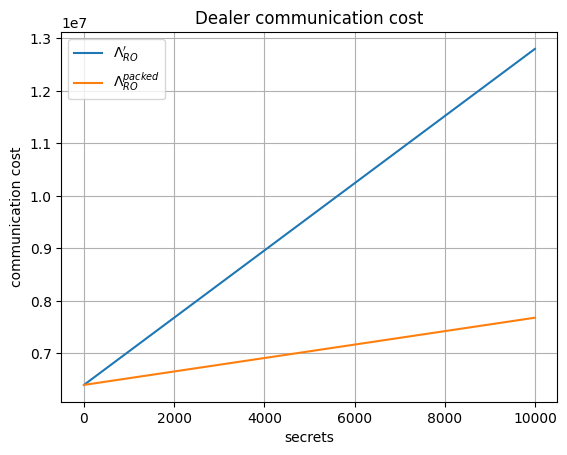
\includegraphics[width=0.7\textwidth]{figures/3pvss_communication_cost.png}
  }
  \caption{This plot compares $\Lambda_{RO}'$ and $\Lambda_{RO}^{packed}$ in terms of communication costs. 
  The x-axis represents the possible number of secrets $\ell$ when the total number of parties 
  is fixed, while the y-axis shows the communication cost for varying $\ell$ and threshold $t$. 
  The blue line corresponds to $\Lambda_{RO}'$, and the orange line corresponds to $\Lambda_{RO}^{packed}$.}
  \label{fig:3pvss_communication_cost}
\end{figure}

In the graph, we fixed the number of parties, $n=10000$, for which we varied $\ell$ with 
$1\leq t\leq \frac{n-\ell}{2}$.

\subsection{On the computational cost}

As $\Lambda_{RO}'$ is a direct extension of $\Lambda_{RO}$ 
\cite{cryptoeprint:2025/576}, the computational 
cost grows linearly with the number of secrets. And as $\Lambda_{RO}^{packed}$ is a slightly 
different approach, we save number of exponentiations in verification by a constant factor of 
$\ell$ but it costs additional group multiplications in share, verification and optiminstic 
reconstruction phases. As group exponentiations with random exponents are usually more 
expensive than group multiplications (to put that in the perspective, computing $g^x$ for 
a random $x\in\mathbb{Z}_q$ can take $\mathcal{O}(\log{q})$ group multiplications). 
Hence, the realistic increase in cost of $\Lambda_{RO}^{packed}$ due to additional 
group multiplications can be negligible. 


\begin{figure}[t!]
  \centering
  \resizebox{\textwidth}{!}{
  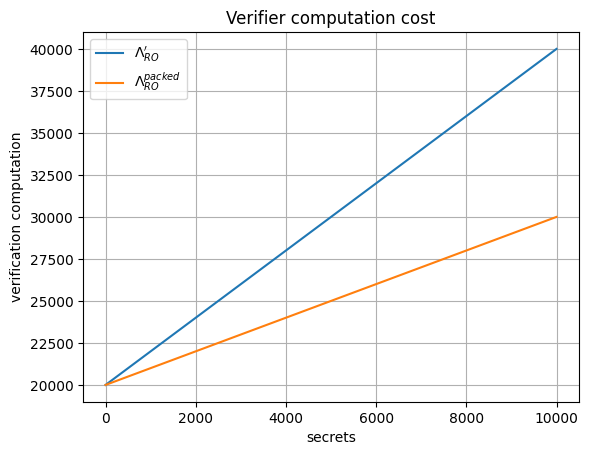
\includegraphics[width=0.7\textwidth]{figures/3pvss_verify_cost.png}
  }
  \caption{This plot compares $\Lambda_{RO}'$ and $\Lambda_{RO}^{packed}$ in terms of computation cost  
  a verifier has to bear in the verification phase. 
  The x-axis represents the possible number of secrets $\ell$ when the total number of parties 
  is fixed, while the y-axis shows the verification cost for varying $\ell$ and threshold $t$. 
  The blue line corresponds to $\Lambda_{RO}'$, and the orange line corresponds to $\Lambda_{RO}^{packed}$.}
  \label{fig:3pvss_verify_cost}
\end{figure}

Similar to the graph in previous subsection, we plotted the speculated computational costs of both the 
schemes in figure \ref{fig:3pvss_verify_cost} where we fixed the number of parties, $n=10000$, 
for which we varied $\ell$ with $1\leq t\leq \frac{n-\ell}{2}$. For this plot, we 
considered the group to be an elliptic curve over a 256-bit prime field which is 
cyclic of order a 256-bit prime $q$, i.e., each element $(x,y)$ on the elliptic curve 
is typically of 512-bit size.\par



% \section{A compact PVSS scheme}
% The relation $\pi_{PDL}^{mod-v1}$ has more potential that a new PVSS can be constructed on top of it. We 
% present it in the figure \ref{fig:compact-PVSS-ro}. 

% \begin{figure}[ht]
    \centering
    \resizebox{\textwidth}{!}{ % Further reduced the scaling factor to fit the content
    \begin{tcolorbox}[title=$\Pi_{S}^{compact}$, width=1.2\textwidth, colframe=blue!75!black, colback=blue!10, sharp corners]
        
        \textbf{Initialization:}
            All parties $\{P_i\}_{i=1}^n$ and dealer $D$ agree on the prime field $\mathbb{Z}_q$, a group 
            $(\mathbb{G},\times)$ of order $q$ with a generator $g$, random oracle $\mathcal{H}$. Also, each party 
            $P_i$ registers their public key $PK_i$ in the public ledger, where $PK_i=g^{SK_i}$ with 
            $SK_i$ being their corresponding secret key.

        \vspace{0.5em}
        \textbf{Share:}
        \begin{itemize}
            \item Dealer $D$ samples a $t$-degree polynomial $f\in\mathbb{Z}_q[X]$ uniformly at random and 
              sets $g^{f_0}$ as secret where $f_0=f(0)$.
            \item For each $1\leq i\leq n$, $D$ encrypts $f(i)=f_i$ with $PK_i$ to obtain 
              $y_i=PK_i^{f_i}$.
            \item $D$ uses $\pi_{PDL}^{AOK}$ \ref{subsec:v1} to generate AoK $\pi_{share}^{AoK}$ to prove that the 
              encryptions are valid, which is done as follows:
            \begin{itemize}
                \item Samples a $t-$degree polynomial $r\in\mathbb{Z}_q[X]$ uniformly at random and 
                computes a single commitment $c=(\prod_{i=1}^{n}PK_i^{r(i)})$.
                \item Using $\mathcal{H}$, $d=\mathcal{H}(y_1,\dots,y_n,c)$ is computed.
                \item Sets $z(X)=r(X)+df(X)$, hence $\pi_{share}^{AoK}=(d,z(X))$ is obtained. 
            \end{itemize}
            \item $D$ broadcasts the encryptions of the shares along with $\pi_{share}^{AoK}$ which 
              proves the validity of the encrypted shares, i.e., broadcasts 
              $\{y_i\}_{i=1}^n$ and $(d,z(X))$.
        \end{itemize}
        
        \vspace{0.5em}
        \textbf{Verification:}
            Given public keys $\{PK_i\}_{i=1}^n$, any entity can check 
            $\pi_{share}^{AoK}$ to verify the correctness of encrypted shares $y_1,\dots,y_n$. 
            They will output \textbf{true} or \textbf{false} based on the verification of the proof. The 
            procedure is outlined as follows:
        \begin{itemize}
            \item The entity checks if $z(X)$ is a $t-$degree polynomial or not.
            \item Checks if $d=\mathcal{H}(y_1,\dots,y_n,\frac{\prod_{i=1}^{n}PK_i^{z(i)}}{[\prod_{i=1}^n y_i]^d})$.
            \item Outputs \textbf{true} if both of the above checks are satisfied, otherwise \textbf{false}.
        \end{itemize}

        \vspace{0.5em}
        \textbf{Reconstruction:}
            Any set $\mathcal{Q}$ consisting $t+1$ honest shareholders will do the following:
            \begin{itemize}
                \item Each party $P_i\in\mathcal{Q}$ decrypts their share $y_i$ using their private key $SK_i$ 
                    corresponding to $PK_i$ to obtain $g^{f_i}$ and then they publish $g^{f_i}$ 
                    along with a DLEQ proof \ref{subsec:chaum-pedersen}, $\pi_{DLEQ}$ which proves that 
                    $g^{f_i}$ is the correct decryption of $y_i$.
                \item They can use the 
                lagrange interpolation to compute the secrets $g^{f_0}$ as follows:
                \begin{align*}
                    g^{f_0} &= \prod_{i\in\mathcal{Q}}(g^{f_i})^{\prod_{k\in\mathcal{Q},k\neq i}\frac{-k}{i}}= g^{\sum_{i\in\mathcal{Q}}f_i\prod_{k\in\mathcal{Q},k\neq i}\frac{-k}{i}}.\\
                \end{align*}
            \end{itemize}
    \end{tcolorbox}
    }
    \caption[PVSS]{$\Pi_{S}^{compact}$, a compact version of $\Pi_{S}$}
    \label{fig:compact-PVSS-ro}
\end{figure}


% \begin{theorem}
%   $\Pi_{S}^{compact}$ is secure.
% \end{theorem}

\section{Conclusion}
In this chapter, we generalized PPVSS to Packed PPVSS and presented two practical schemes based on 
Packed Shamir secret sharing. The reason to introduce the 3PVSS $\Lambda_{RO}'$ is because of its 
potential applications in some e-voting protocols. In this thesis, we wanted to mainly focused on randomness beacon 
protocols based on PVSS, due to this reason we introduced our second 3PVSS $\Lambda_{RO}^{packed}$ which is based on the
NIZK AoK $\pi_{mod-PDL}^{AoK}$ for the modified-PDL problem.\par

In the next chapter, we will revisit the randomness beacon ALBATROSS \cite{cryptoeprint:2020/644} based on PVSS, 
and replace the Packed Shamir secret sharing based PVSS with our 3PVSS $\Lambda_{RO}^{packed}$. 

%%% Local Variables: 
%%% mode: latex
%%% TeX-master: "thesis"
%%% End: 

% ... and so on until
\chapter{Revisiting a Randomness Beacon Protocol}
\label{cha:n}

Randomness Beacon \cite{RABIN1983256} is required in applications like e-voting \cite{10.5555/1496711.1496734} 
and anonymous messaging (\cite{180263},\cite{10.1145/2815400.2815417}) to provide fresh random values to all the 
parties. In 2020, Cascudo and David published ALBATROSS \cite{cryptoeprint:2020/644}, the state-of-the art randomness 
beacon protocol based on a PVSS as a building block where each party in the randomness beacon protocol acts as a dealer once, so that all 
parties can influence the output randomness. Interestingly, we observed that each party is expected to reveal 
their secrets (they secret shared as a dealer) as part of the randomness beacon protocol, but to prove that the 
secrets are valid and not just some random evaluations of the secret polynomial they have to reveal the whole 
secret polynomial itself. As a consequence, if some entity wants to verify the secrets' validity then they have to 
simulate the whole sharing phase of the underlying PVSS protocol, which is very expensive because all the rest of the 
parties are expected to do the simulation of that party as a dealer. For reference, if there are $n$ parties, then 
$n-1$ parties should simulate the sharing phase of the protocol, which in total is $\mathcal{O}(n^2)$ simulations.\par

In this chapter, we present our randomness beacon protocol in figures \ref{fig:randomness_beacon} and \ref{fig:randomness_beacon_cont} 
which in many cases is efficient than ALBATROSS. To put simply, we replaced the building block being PVSS with 
our PPPVSS $\Lambda_{RO}^{packed}$ \ref{fig:packed-shamir-PPPVSS-ro}. In the subsequent sections, we will discuss the 
computational and communication costs of our protocol and compare it with the ALBATROSS. We will show that out protocol 
performs more efficient compared to ALBATROSS in many cases and also address the cases where we are not computationally efficient.
More interestingly, we will show that in terms of communication, we outperform ALBATROSS.

\begin{figure}[ht]
    \centering
    \begin{tcolorbox}[title=\textbf{Randomness Beacon using PPPVSS}, width=0.9\textwidth, colframe=blue!75!black, colback=blue!10, sharp corners]
        Our protocol with PPPVSS is run between a set $\mathcal{P}$ of $n$ 
        parties $P_1, \dots, P_n$ who have access to a public ledger where they 
        can post information for later verification. It is assumed that the 
        Setup phase of $\Pi_{PPPVSS}$ is already done and the public keys 
        $\text{pk}_i$ of each party $P_i$ along with $\{\mathbb{P}_i\}_{i=1}^{l}$ 
        being Commitment keys (or public keys of target people) to encrypt the 
        $l$ secrets are already registered in the ledger. In addition, the 
        parties have agreed on a Vandermonde $(n - 2t) \times (n - t)$-matrix 
        $M = M(\omega, n - 2t, n - t)$ with $\omega \in \mathbb{Z}_q^*$.

    \begin{enumerate}
        \item [1.]\textbf{Commit:} For $1 \leq j \leq n$:
        \begin{itemize}
            \item Shareholder $P_j$ executes the Distribution phase of the 
            PPPVSS as Dealer for $\ell = n - 2t$ secrets, publishing commitments 
            (/encryptions) of secrets, $y_{-(l-1)}^j, \dots, y_{-1}^j, y_0^j$, 
            and encryptions of shares $\{y_i^j\}_{i=1}^n$ along with 
            $\pi_{proof}^{j}$, which is a NIZK PoK for proving the correctness of 
            committed(/encrypted) secrets and encrypted secret shares on the 
            public ledger, also learning the secrets $h^{s_0^j},...,h^{s_{-(l-1)}^j}$ 
            and their corresponding exponents\\ $s_0^j, \dots, s_{-(l-1)}^j$.
        \end{itemize}
        
        \item [2.]\textbf{Reveal:}
        \begin{itemize}
            \item Each shareholder checks the validity of the proof 
            $\pi_{proof}^j$, i.e., the \textbf{verification phase of PPPVSS protocol}.
            \item After a set $\mathcal{C}$ containing at least $n-t$ 
            shareholders publish their shares in the public ledger, 
            $P_j\in\mathcal{C}$ reveals $l$ secrets.
            \item Every shareholder verifies the validity of secrets by 
            reproducing the commitments using the commitment keys (/public keys 
            of target people).
            \item At this point, if every party in $\mathcal{C}$ has opened 
            their secrets correctly, go to step 4' in Figure \ref{fig:9}. 
            Otherwise, proceed to step 3 in Figure \ref{fig:9}.
        \end{itemize}
    \end{enumerate}
    \end{tcolorbox}
    \caption{Commit and Reveal phase of the Randomness Beacon using PPPVSS}
    \label{fig:randomness_beacon}
\end{figure}
\begin{figure}[t!]
    \centering
    \begin{tcolorbox}[title=\textbf{Randomness Beacon using 3PVSS, $\Lambda_{RO}^{packed}$ (cont.)}, width=0.9\textwidth, colframe=blue!75!black, colback=blue!10, sharp corners]
        \begin{enumerate}
            \item [3.]\textbf{Recovery:} Let $\mathcal{C}_a$ be the set containing at most $t$ malicious shareholders(as Dealers) who did not open the exponents corresponding to their $\ell$ secrets, $\{h^{s_i^k}\}_{i=0}^{-(\ell-1)}$ for each $P_k\in\mathcal{C}_a$, in \textit{Reveal} phase.
            \begin{itemize}
                \item Every shareholder $P_j$ should decrypt the secret share of each malicious shareholder(Dealer) in $\mathcal{C}_a$, and give a DLEQ proof \ref{subsec:chaum-pedersen} which asserts that the decryption is performed correctly,i.e., each shareholder should perform the \textit{pessimistic} reconstruction phase of the 3PVSS $\Lambda_{RO}^{packed}$ for every shareholder(Dealer) who has not revealed the exponents corresponding to their secrets.
            \end{itemize}
            
            \item [4]\textbf{Output:}  Let $T$ be the $(n - t) \times \ell$ matrix with rows indexed by the shareholders in $\mathcal{C}$ and where the row corresponding to $P_a \in \mathcal{C}$ is $(h^{s_0^a} , . . . , h^{s_{-(\ell-1)}^a})$.
            \begin{itemize}
                \item Each computes the $\ell \times \ell$-matrix $R = M \circ T$ by applying FFTE to each column $T^{(j)}$ of $T$, resulting in column $R^{(j)}$ of $R$ (since $R^{(j)} = M \circ T^{(j)}$ and $M$ is Vandermonde) for $j \in [0, \ell - 1]$.
                \item Shareholders output the $\ell^2$ elements of $R$ as final randomness.
            \end{itemize}
        
            \item [4']\textbf{Alternative Output:}  if every party in $\mathcal{C}$ has opened her secrets correctly in step \textit{Reveal}, then:
            \begin{itemize}
                \item Shareholders compute $R = M \circ T$ in the following way:\\
                    Let $S$ be the $(n - t) \times \ell$ matrix with rows indexed by the shareholders in $\mathcal{C}$ and where the row
                    corresponding to $P_a \in\mathcal{C}$ is $(s_0^a,...,s_{-(\ell-1)}^a )$. Then each party computes $U = M \circ S \in\mathbb{Z}_q^{\ell\times \ell}$ (using the standard FFT in $\mathbb{Z}_q$ to compute each column) and $R = h^U$ .
                \item Shareholders output the $\ell^2$ elements of $R$ as final randomness.
            \end{itemize}
        \end{enumerate}
    \end{tcolorbox}
    \caption{Recovery and Output phase of the Randomness Beacon using 3PVSS}
    \label{fig:randomness_beacon_cont}
\end{figure}
\section{Computational Complexity}
\begin{table}[H]
\centering
\begin{tabular}{|p{3cm}|p{1.2cm}|p{2.5cm}|p{5.5cm}|p{2.5cm}|}
\hline
\textbf{Protocol}    & \textbf{Output size}    & 
\textbf{Commit}\textit{(by Dealer)} & \textbf{Reveal}\textit{(by 
shareholder)} & \textbf{Recovery} \textit{(by shareholder)}                                                           
\\ \hline
\textbf{ALBATROSS}, \textit{Honest case}    & $l^2$ & 
$(2n+l)[\mathbb{E}_x+\mathbb{P}_e]$ & \textbf{Share Verification - }  &  
\\
& & & $(n-1)n[2\mathbb{E}_x+\mathbb{P}_e]$ & \\
& & & \textbf{Secret Verification - } & \\ 
& & & $(n-1)(n+l)[\mathbb{E}_x+\mathbb{P}_e]$&- \\ \hline
\textbf{with PPPVSS}, \textit{Honest case}    & $l^2$  & 
$2(n+l)[\mathbb{E}_x+\mathbb{P}_e]$ & \textbf{Share Verification - } &  \\ 
& & & $(n-1)(n+l)[2\mathbb{E}_x+\mathbb{P}_e]$ &  \\ 
& & & &  \\
& & & \textbf{Secret Verification - } & \\ 
& & & $(n-1)l\mathbb{E}_x$ & -  \\ \hline
\textbf{ALBATROSS}, \textit{Robust case}    & $l^2$ & 
$(2n+l)[\mathbb{E}_x+\mathbb{P}_e]$ & \textbf{Share Verification - }  &  
\\
& & & $(n-1)n[2\mathbb{E}_x+\mathbb{P}_e]$ & \\
& & & \textbf{Secret Verification - } & \\ 
& & & $(n-t-1)(n+l)[\mathbb{E}_x+\mathbb{P}_e]$& 
$[3+4(n-t)]t\mathbb{E}_{x}$\\ \hline
\textbf{with PPPVSS}, \textit{Robust case}    & $l^2$  & 
$2(n+l)[\mathbb{E}_x+\mathbb{P}_e]$ & \textbf{Share Verification - } &  \\ 
& & & $(n-1)(n+l)[2\mathbb{E}_x+\mathbb{P}_e]$ &  \\
& & & \textbf{Secret Verification - } & \\ 
& & & $(n-t-1)l\mathbb{E}_x$ &   \\
& & & & $[3+4(n-t)]t\mathbb{E}_{x}$  \\ \hline

\end{tabular}
\caption{Computational cost of dealer and shareholders, 
$\mathbb{E}_x=$group exponentiation and $\mathbb{P}_e=$polynomial 
evaluation in group $G$ with order $q$, where $q$ is a large prime}
\label{tab:comp_alba_pppvss_no group mul}
\end{table}


See table \ref{tab:comp_alba_pppvss_no group mul} for an overview.
\begin{itemize}
    \item In ALBATROSS, a dealer(as a part of \textbf{commit}) should compute $n(\mathbb{E}_x+\mathbb{P}_e)$ commitments and to give a proof he should do an additional $n(\mathbb{P}_{e}+\mathbb{E}_{x})$. Also, on dealer should do $l(\mathbb{P}_e+\mathbb{E}_x)$ for computing secrets and keeping it to himself. In total dealer needs to do $(2n+l)[\mathbb{E}_x+\mathbb{P}_{e}]$.
        \begin{itemize}
            \item In \textbf{Reveal}, a verifier should compute $2n\mathbb{E}_{x}$ which internally requires additional $n\mathbb{P}_{e}$, i.e., in total it requires $(n-1)n(2\mathbb{E}_{x}+\mathbb{P}_{e})$ computations for each verifier.
            \begin{itemize}
                \item In \textbf{Robust case} where $t$ dealers do not open their polynomials, a verifier should verify $n-t$ polynomials of honest dealers, i.e., for each honest dealer, a verifier has to do $n\mathbb{P}_e$ to evaluate secret share exponents and does $n\mathbb{E}_x$ to get secret shares and cross checks them in the public ledger. Also, finally the verifier computes $l\mathbb{P}_e$ to get secret exponents and get $l$ secrets by doing $l\mathbb{E}_x$. As there are $n-t$ honest dealers, the verifier has to compute $(n-t)(n+l)(\mathbb{E}_x+\mathbb{P}_e)$.
                \item  In \textbf{Honest case}, everyone would have been honest and so each verifier has to do $(n-1)(n+l)(\mathbb{E}_x+\mathbb{P}_e)$.
            \end{itemize}
            \item \textbf{Recovery} phase only exists if some party does not 
            open the polynomial leading to PVSS reconstruction phase, in the 
            worst case there should be reconstruction for the secrets of $t$ 
            malicious parties. Given a malicious shareholder who has not opened 
            the secret polynomial, each shareholder/re-constructor has to 
            decrypt their share, which requires $1\mathbb{E}_{x}$ and should 
            give a DLEQ proof that they have decrypted correctly, which 
            additionally requires $2\mathbb{E}_x$; Also the re-constructor 
            should verify DLEQ proofs of correct share decryption from $n-t$ 
            honest shareholders requiring them to do $4(n-t)\mathbb{E}_{x}$. 
            In total, each re-constructor requires $[3+4(n-t)]t\mathbb{E}_{x}$.
        \end{itemize}
    \item Using PPPVSS in randomness beacon protocol, a dealer(as a part of \textbf{commit}) requires to do $(n+l)[\mathbb{E}_x+\mathbb{P}_e]$ and $(l-1)\mathbb{M}_G$ to compute $\{y_i\}_{i=0}^{n}$. For generating the proof that $y_i$'s are valid encryptions of the secret shares and also $y_0$ is a commitment of the $l$ secrets, the dealer should do $(n+l)[\mathbb{E}_x+\mathbb{P}_e]$ which internally requires additional $(l-1)\mathbb{M}_G$. In total, a dealer has to do $2\left[(n+l)[\mathbb{E}_x+\mathbb{P}_e]+(l-1)\mathbb{M}_{G}\right]$.
    \begin{itemize}
        \item In \textbf{Reveal}, a verifier should do $(n+l)(2\mathbb{E}_x+\mathbb{P}_e)$ and $(l-1)\mathbb{M}_G$ for each proof. In total, a verifier has to do $(n-1)(n+l)[2\mathbb{E}_x+\mathbb{P}_e]+(n-1)(l-1)\mathbb{M_G}$.
        \begin{itemize}
            \item In \textbf{Robust case} with $t$ malicious parties not opening the secret polynomials, a verifier should do $l\mathbb{E}_x+(l-1)\mathbb{M}_G$ to verify each proof, so in total each verifier should do $(n-t-1)[l\mathbb{E}_x+(l-1)\mathbb{M}_G]$.
            \item In \textbf{Honest case} where everyone is honest, a verifier will do $(n-1)l(\mathbb{E}_x+\mathbb{M}_G)$.
        \end{itemize}
        \item The computational complexity of each re-constructor in \textbf{Recovery} phase is exactly same as in the case of ALBATROSS.
    \end{itemize}
\end{itemize}

\subsection{Computational Cost analysis}
The dealer has to do a bit more work in the case of our protocol in contrast to ALBATROSS, more explicitly, 
they have to compute $\ell$ more group exponentiations and polynomial evaluations. But as a consequence, 
we decrease computational cost in the \textit{Reveal} phase whenever $l < \frac{n(n-t-1)}{2(n-1)}$, roughly 
speaking, if the number of secrets are less than half of the honest parties then we always perform better in 
terms of computation when compared to the ALBATROSS.


\section{Communication Complexity}
\begin{table}[H]
\centering
\begin{tabular}{|p{3cm}|p{4cm}|p{3.5cm}|p{4cm}|p{1cm}|}
\hline
\textbf{Protocol}     & \textbf{Commit} \textit{(by Dealer)} & \textbf{Reveal} \textit{(by Dealer)} & \textbf{Recovery}  \textit{(by shareholder)}                                                      \\ \hline
\textbf{ALBATROSS}   & $nG+(t+l)\mathbb{Z}_q$ & $(t+l)\mathbb{Z}_q$ & $1G+1\mathbb{Z}_q+1R_o$ \\ \hline
\textbf{with PPPVSS}    & $(n+1)G+(t+l)\mathbb{Z}_q$ & $l\mathbb{Z}_q$ & $1G+1\mathbb{Z}_q+1R_o$ \\ \hline

\end{tabular}
\caption{Communication cost of dealer and (each) shareholder, $R_o$ being the random oracle, $G = $group of order $q$ and $\mathbb{Z}_q =$ modular group of order $q$, where $q$ is a large prime}
\label{tab:dealer_comm}
\end{table}

See table \ref{tab:dealer_comm} for an overview.
\begin{itemize}
    \item In ALBATROSS, a dealer (as a part of \textbf{commit}) should send $n$ group elements as commitments, $t+l$ elements in $\mathbb{Z}/q\mathbb{Z}$ that defines the polynomial used in the ZKP and $1$ extra element in $\mathbb{Z}/q\mathbb{Z}$ from RO. 
    \begin{itemize}
        \item In \textbf{Reveal}, an honest dealer would broadcast $t+l$ coefficients in $\mathbb{Z}/q\mathbb{Z}$ concerning the secret polynomial.
        \item If some party has not revealed their polynomial, then in \textbf{Recovery} phase a re-constructor using PVSS reconstruction protocol should broadcast $1$ element in group which is being the decrypted secret, for the proof of correct decryption, they have to broadcast $3$ more group elements along with a polynomial which requires $t+l$ coefficients in $\mathbb{Z}/q\mathbb{Z}$ and $1$ group element from RO.
    \end{itemize}
    \item Using PPPVSS in randomness beacon protocol, a dealer (as a part of \textbf{commit}) should send $n+1$ group elements as commitments, $t+l$ elements in $\mathbb{Z}/q\mathbb{Z}$ that defines the polynomial used in the ZKP and $1$ extra element in $\mathbb{Z}/q\mathbb{Z}$ from RO.
    \begin{itemize}
        \item In \textbf{Reveal}, an honest dealer would broadcast $l$ elements in $\mathbb{Z}_q$ concerning the exponents to construct the secret.
        \item If some part has not revealed their secrets, then the communication cost of each re-constructor is exactly same as in the case of ALBATROSS.
    \end{itemize}
\end{itemize}

\subsection{Communication Cost analysis}
The best to offer from our randomness beacon protocol is the communication cost. Though the dealer has to communicate only 
one extra group element compared to ALBATROSS in the commit phase, as a consequence for a fixed number of secrets the 
dealers' communication cost is constant as opposed to linear in number of corrupted parties in ALBATROSS. 

%%% Local Variables: 
%%% mode: latex
%%% TeX-master: "thesis"
%%% End: 

\chapter{Conclusion}
\label{cha:conclusion}
The final chapter contains the overall conclusion. It also contains
suggestions for future work and industrial applications.


%%% Local Variables: 
%%% mode: latex
%%% TeX-master: "thesis"
%%% End: 


% % If you have appendices:
% \appendixpage*          % if wanted
% \appendix
% \chapter{The First Appendix}
\label{app:A}
Appendices hold useful data which is not essential to understand the work
done in the master's thesis. An example is a (program) source.
An appendix can also have sections as well as figures and references\cite{h2g2}.

\section{More Lorem}
\lipsum[50]

\subsection{Lorem 15--17}
\lipsum[15-17]

\subsection{Lorem 18--19}
\lipsum[18-19]

\section{Lorem 51}
\lipsum[51]

%%% Local Variables: 
%%% mode: latex
%%% TeX-master: "thesis"
%%% End: 

% % ... and so on until
% \chapter{The Last Appendix}
\label{app:n}
Appendices are numbered with letters, but the sections and subsections use
arabic numerals, as can be seen below.

\section{Lorem 20-24}
\lipsum[20-24]

\section{Lorem 25-27}
\lipsum[25-27]

%%% Local Variables: 
%%% mode: latex
%%% TeX-master: "thesis"
%%% End: 


\backmatter
% The bibliography comes after the appendices.
% You can replace the standard "abbrv" bibliography style by another one.
\bibliographystyle{abbrv}
\bibliography{references}

\end{document}